\UseRawInputEncoding
\documentclass[hyperref={pdfpagelabels=false}]{beamer}
% Die Hyperref Option hyperref={pdfpagelabels=false} verhindert die Warnung:
% Package hyperref Warning: Option `pdfpagelabels' is turned off
% (hyperref)                because \thepage is undefined. 
% Hyperref stopped early 
%

\usepackage{lmodern}
% Das Paket lmodern erspart die folgenden Warnungen:
% LaTeX Font Warning: Font shape `OT1/cmss/m/n' in size <4> not available
% (Font)              size <5> substituted on input line 22.
% LaTeX Font Warning: Size substitutions with differences
% (Font)              up to 1.0pt have occurred.
%

% Wenn \titel{\ldots} \author{\ldots} erst nach \begin{document} kommen,
% kommt folgende Warnung:
% Package hyperref Warning: Option `pdfauthor' has already been used,
% (hyperref) ... 
% Daher steht es hier vor \begin{document}

\title[Simon Kl{\"u}ttermann]{Anomaly detection in physics}   
\author{Simon Kluettermann} 
\date{\today} 




% Dadurch wird verhindert, dass die Navigationsleiste angezeigt wird.
\setbeamertemplate{navigation symbols}{}

% zusaetzlich ist das usepackage{beamerthemeshadow} eingebunden 
\usepackage{beamerthemeshadow}

\hypersetup{pdfstartview={Fit}} % fits the presentation to the window when first displayed

\usepackage{appendixnumberbeamer}

\usetheme{CambridgeUS}
\usepackage{ngerman}
\usecolortheme{dolphin}


%  \beamersetuncovermixins{\opaqueness<1>{25}}{\opaqueness<2$\Rightarrow${15}}
%  sorgt dafuer das die Elemente die erst noch (zukuenftig) kommen 
%  nur schwach angedeutet erscheinen 
%\beamersetuncovermixins{\opaqueness<1>{25}}{\opaqueness<2$\Rightarrow${15}}%here disabled
% klappt auch bei Tabellen, wenn teTeX verwendet wird\ldots
\renewcommand{\figurename}{}

\setbeamertemplate{footline}
{
  \leavevmode%
  \hbox{%
  \begin{beamercolorbox}[wd=.4\paperwidth,ht=2.25ex,dp=1ex,center]{author in head/foot}%
    \usebeamerfont{author in head/foot}\insertshorttitle
  \end{beamercolorbox}%
  \begin{beamercolorbox}[wd=.25\paperwidth,ht=2.25ex,dp=1ex,center]{title in head/foot}%
    \usebeamerfont{title in head/foot}\insertsection
  \end{beamercolorbox}%
  \begin{beamercolorbox}[wd=.3499\paperwidth,ht=2.25ex,dp=1ex,right]{date in head/foot}%
    \usebeamerfont{date in head/foot}\insertshortdate{}\hspace*{2em}
    \hyperlink{toc}{\insertframenumber{} / \inserttotalframenumber\hspace*{2ex}} 
  \end{beamercolorbox}}%
  \vskip0pt%
}

\usepackage[absolute,overlay]{textpos}
\usepackage{graphicx}

\newcommand{\source}[1]{\begin{textblock*}{9cm}(0.1cm,8.9cm)
    \begin{beamercolorbox}[ht=0.5cm,left]{framesource}
        \usebeamerfont{framesource}\usebeamercolor[fg!66]{framesource} Source: {#1}
    \end{beamercolorbox}
\end{textblock*}}


\begin{document}



%from file ../oan/presentation//data/00title
\begin{frame}[label=]
\frametitle{}
\titlepage
\end{frame}



%from file ../oan/presentation//data/01tt
\newpage
\section{Anomalies and Physics}\label{sec:Anomalies and Physics}
%{{{for_Anomalies and Physics}}}


\begin{frame}[label=]
\frametitle{}
\begin{figure}[H] 
  \centering
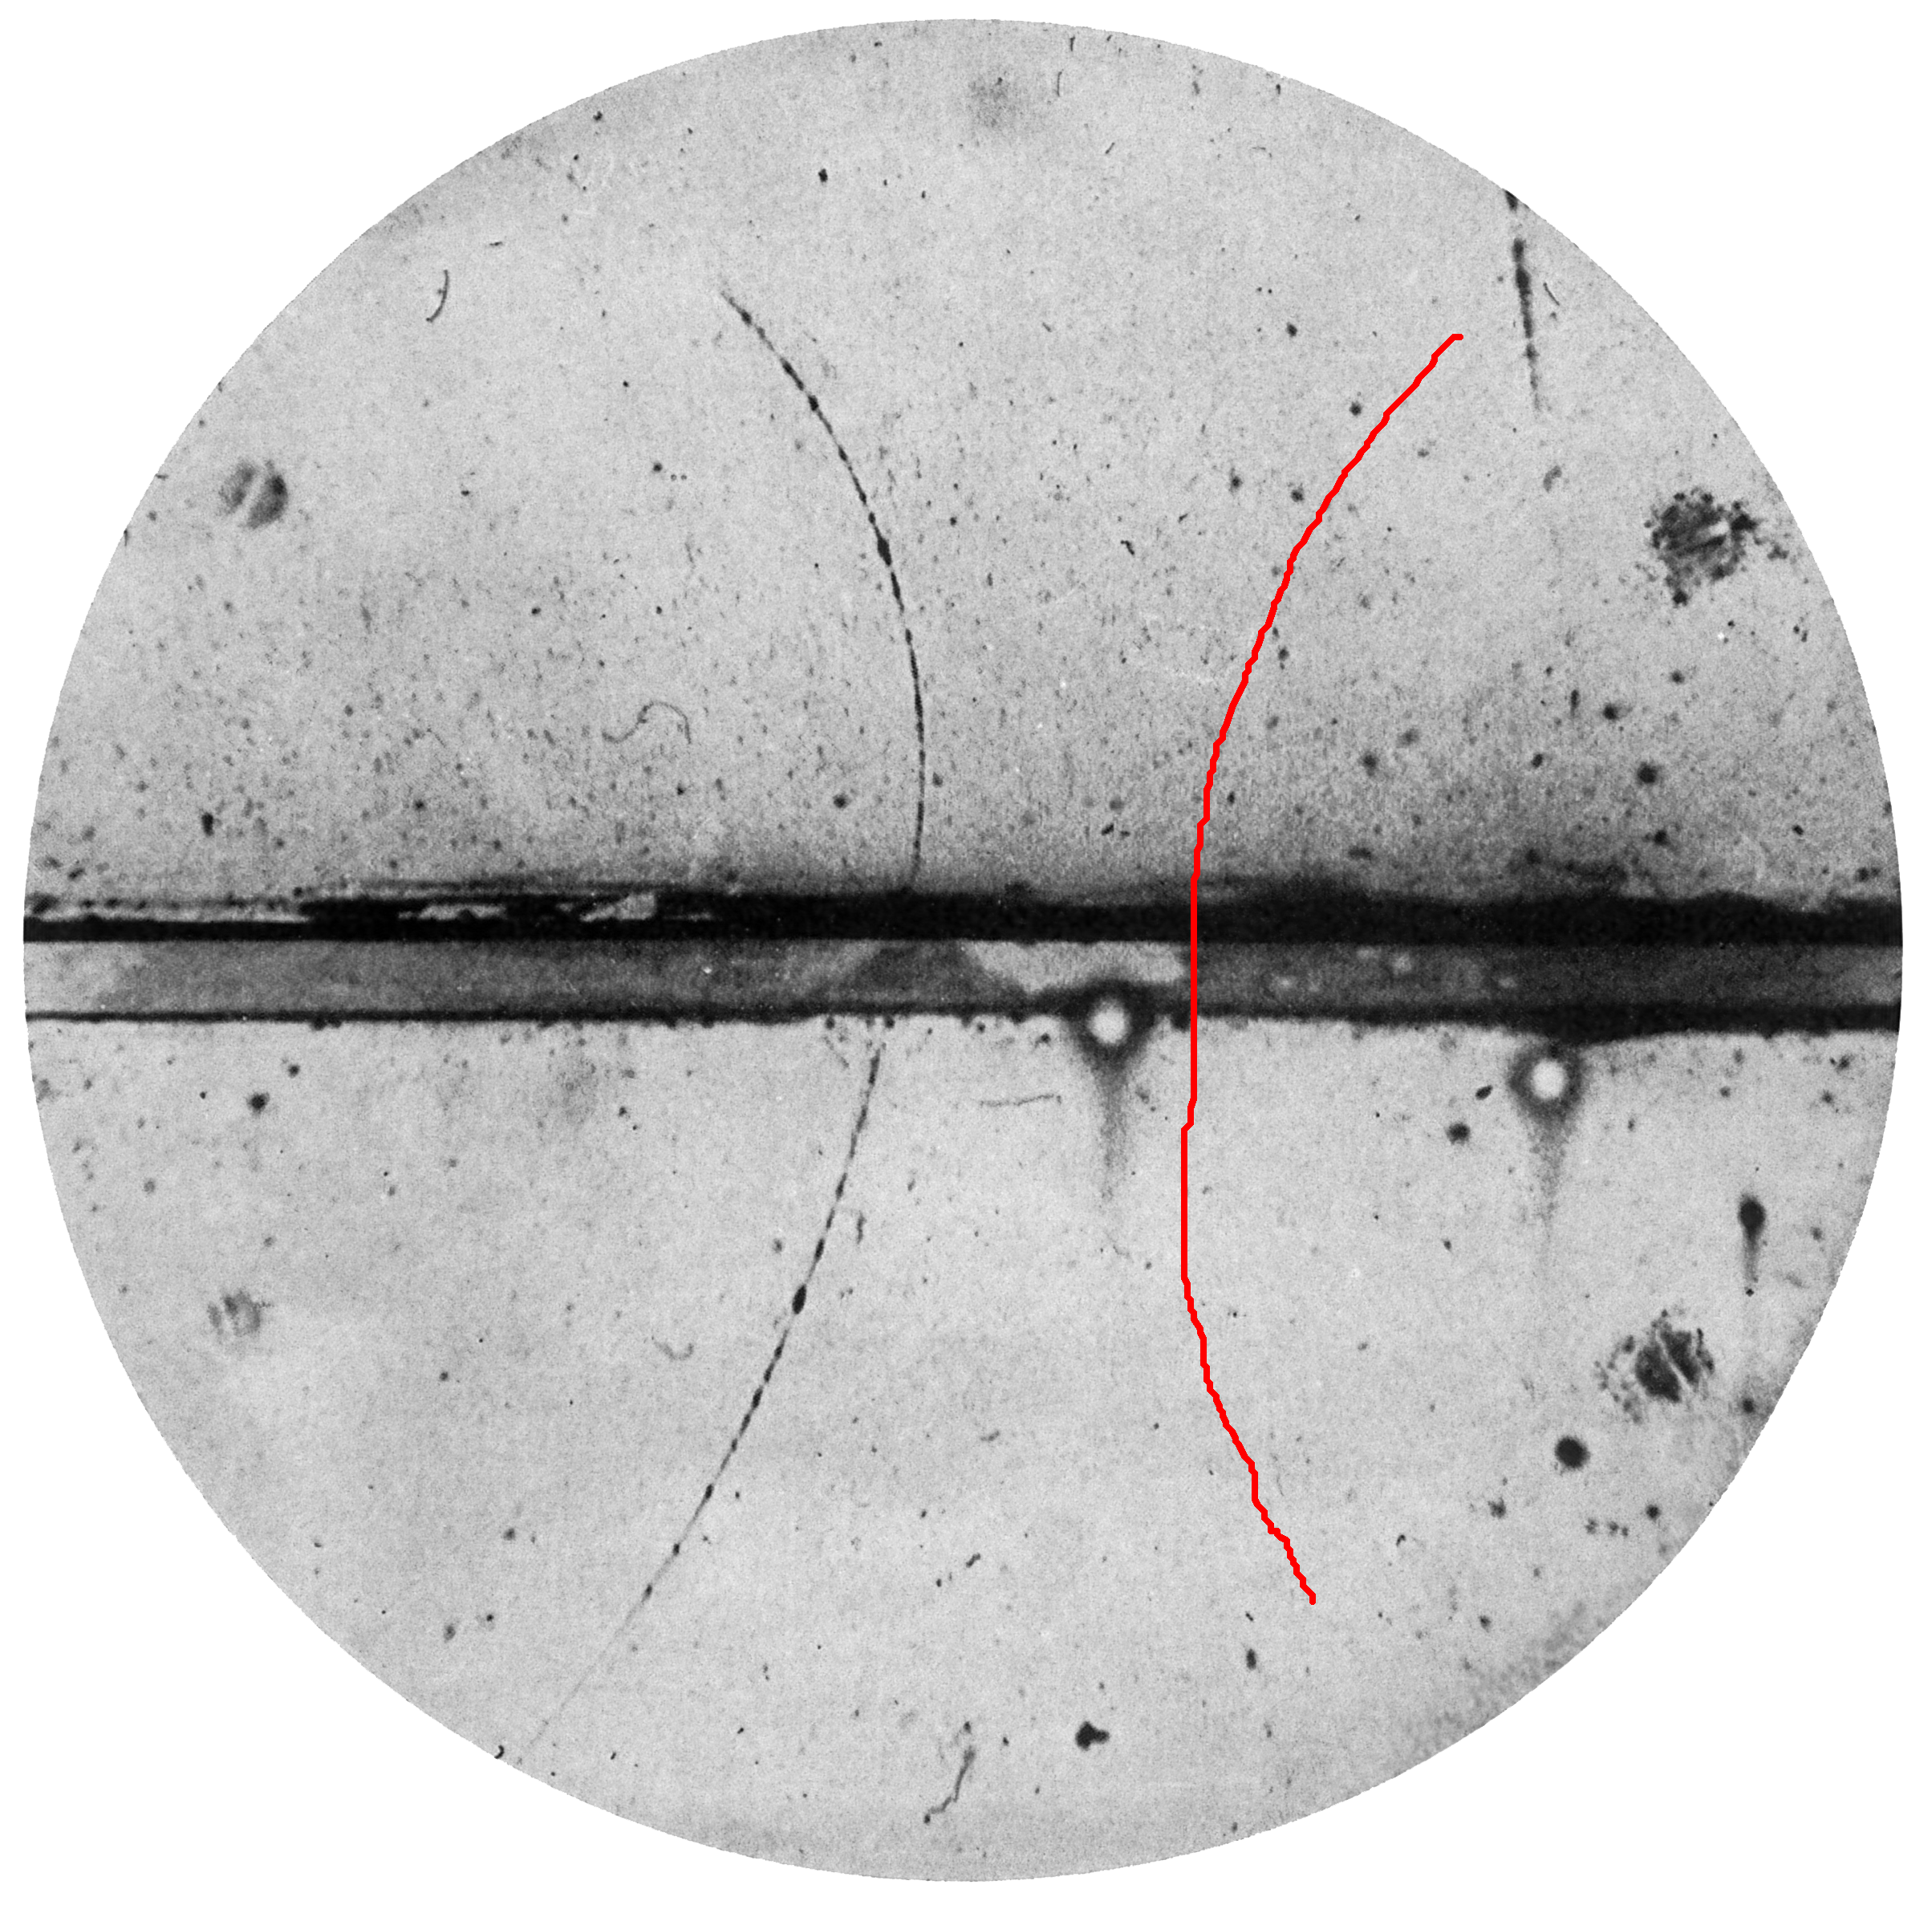
\includegraphics[height=0.9\textheight]{../imgs/positron2.png}
\label{fig:positron2png}
  \end{figure}


\end{frame}

\begin{frame}[label=]
\frametitle{}
\begin{figure}[H] 
  \centering
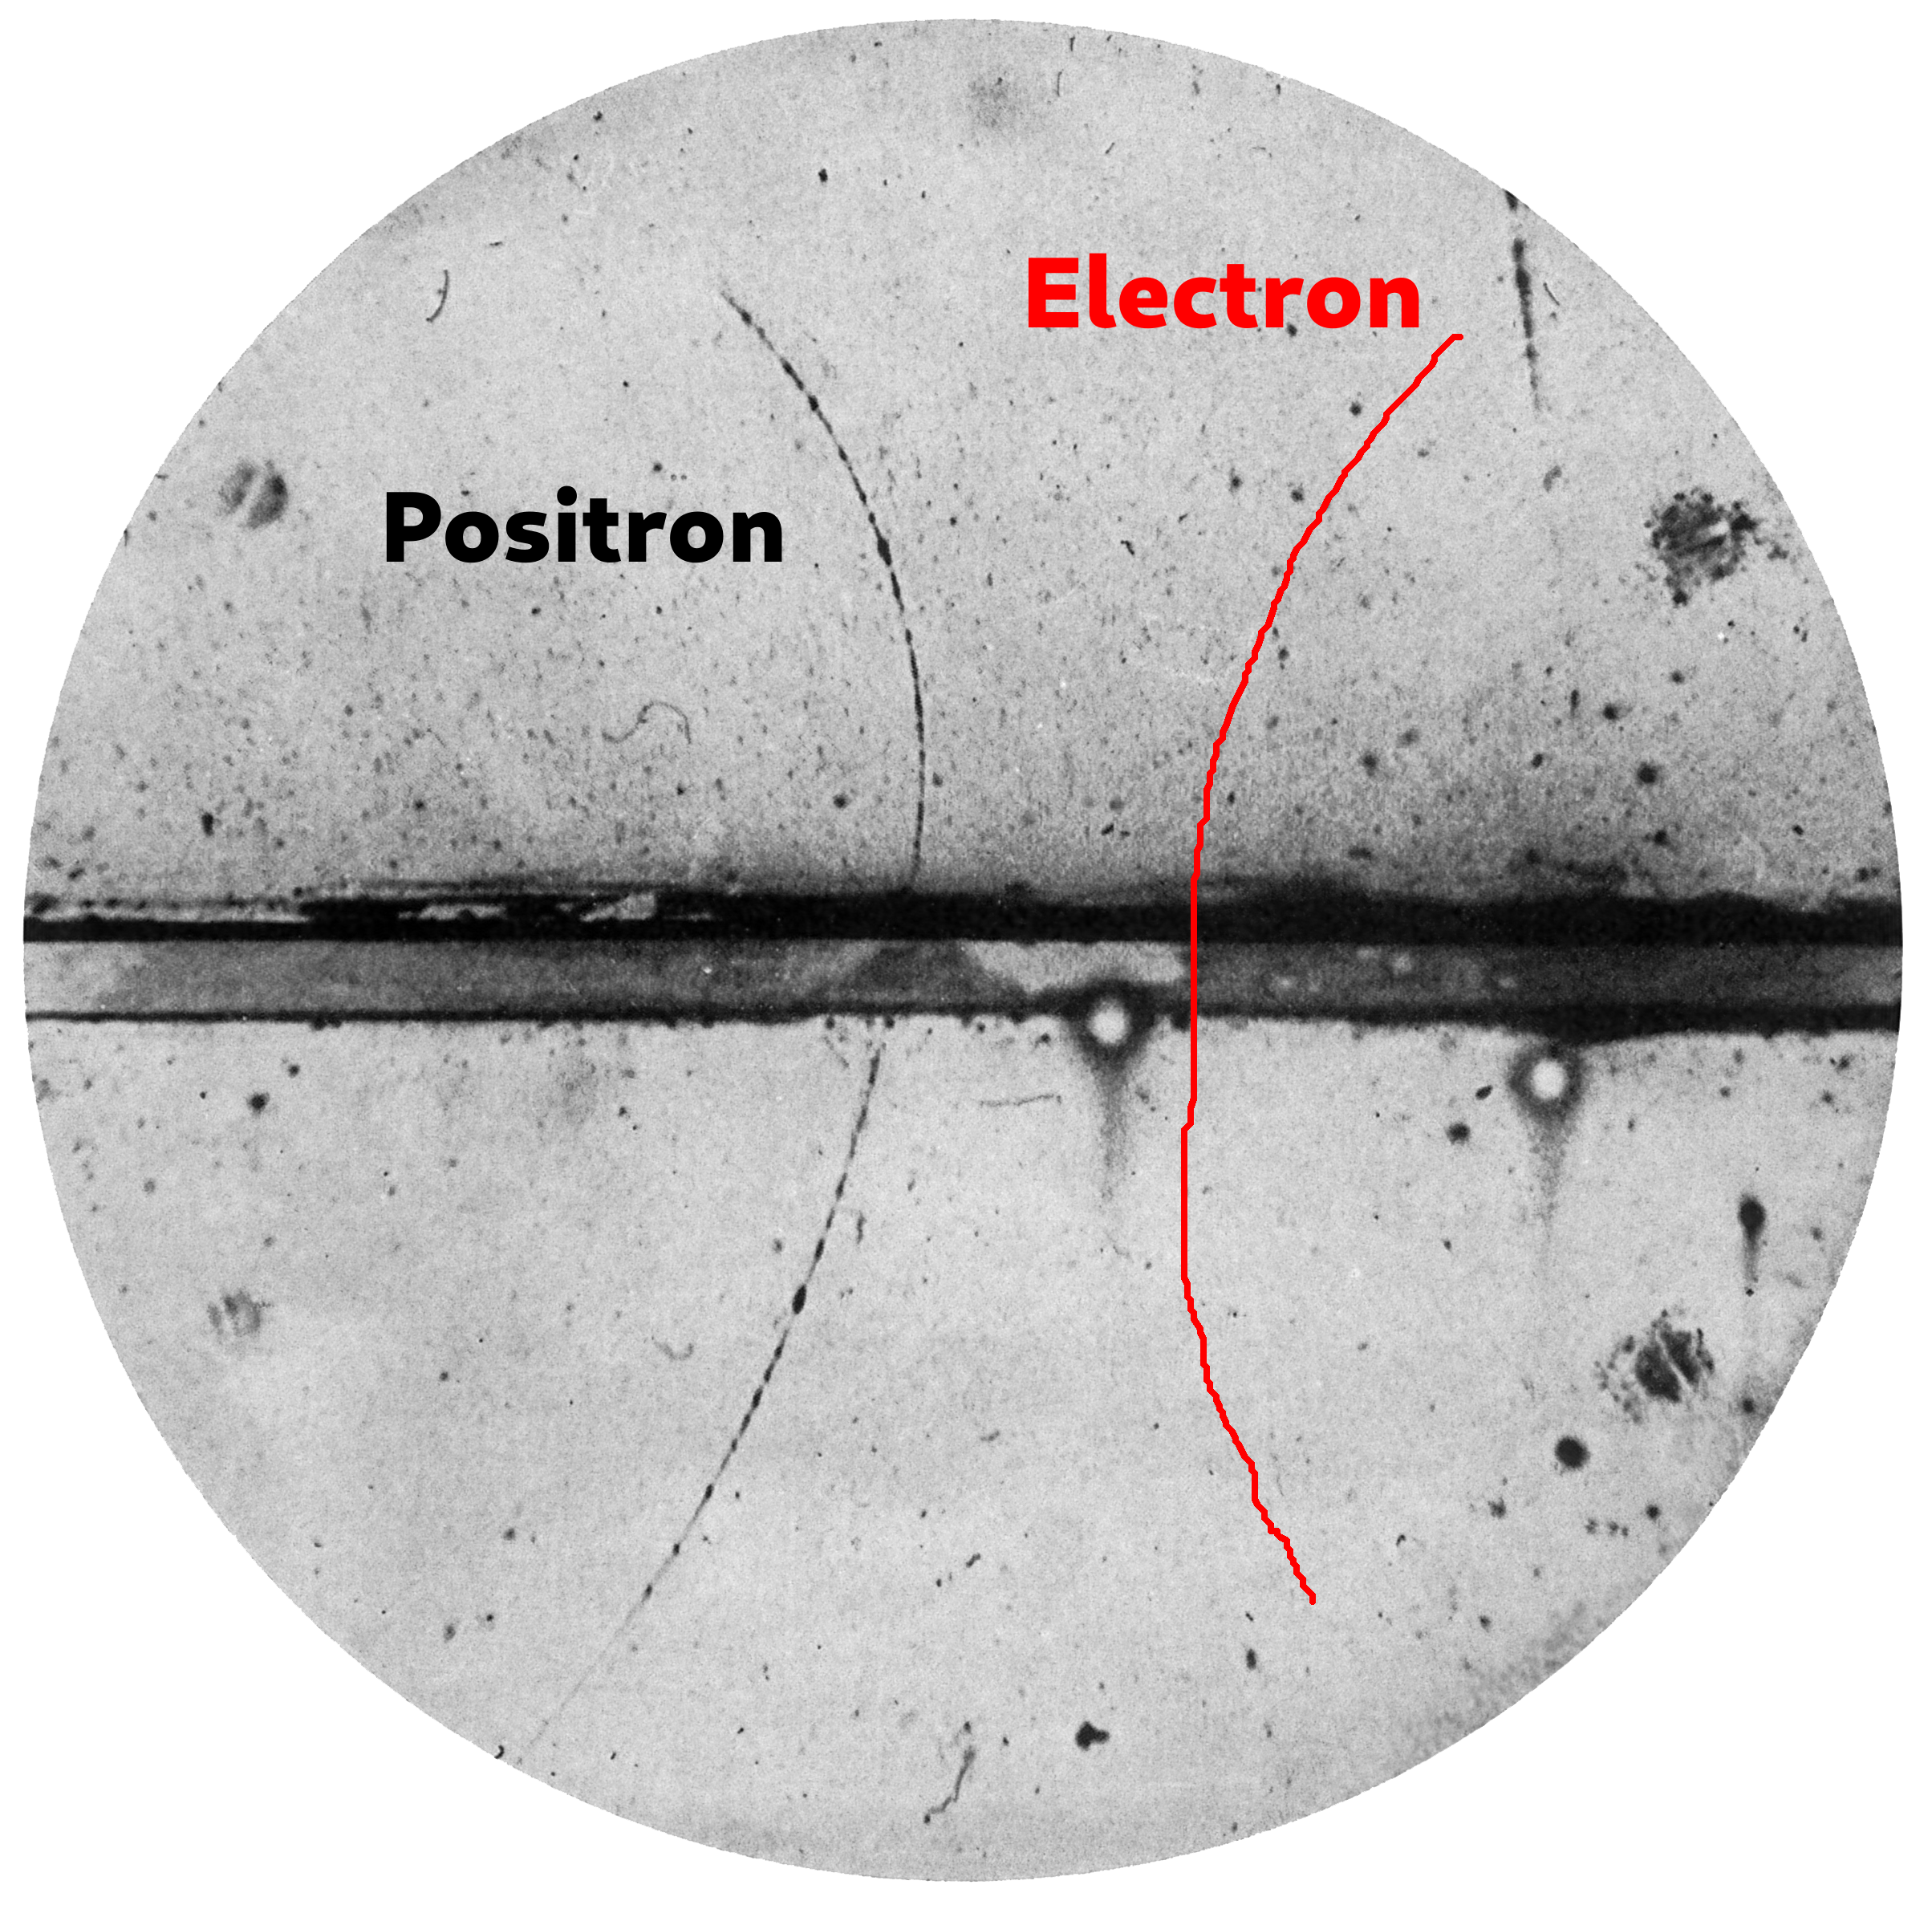
\includegraphics[height=0.9\textheight]{../imgs/positron3.png}
\label{fig:positron3png}
  \end{figure}


\end{frame}

\begin{frame}[label=]
\frametitle{}
\begin{textblock*}{5cm}(0cm,0.2cm) % {block width} (coords)
\begin{figure}[H] 
  \centering
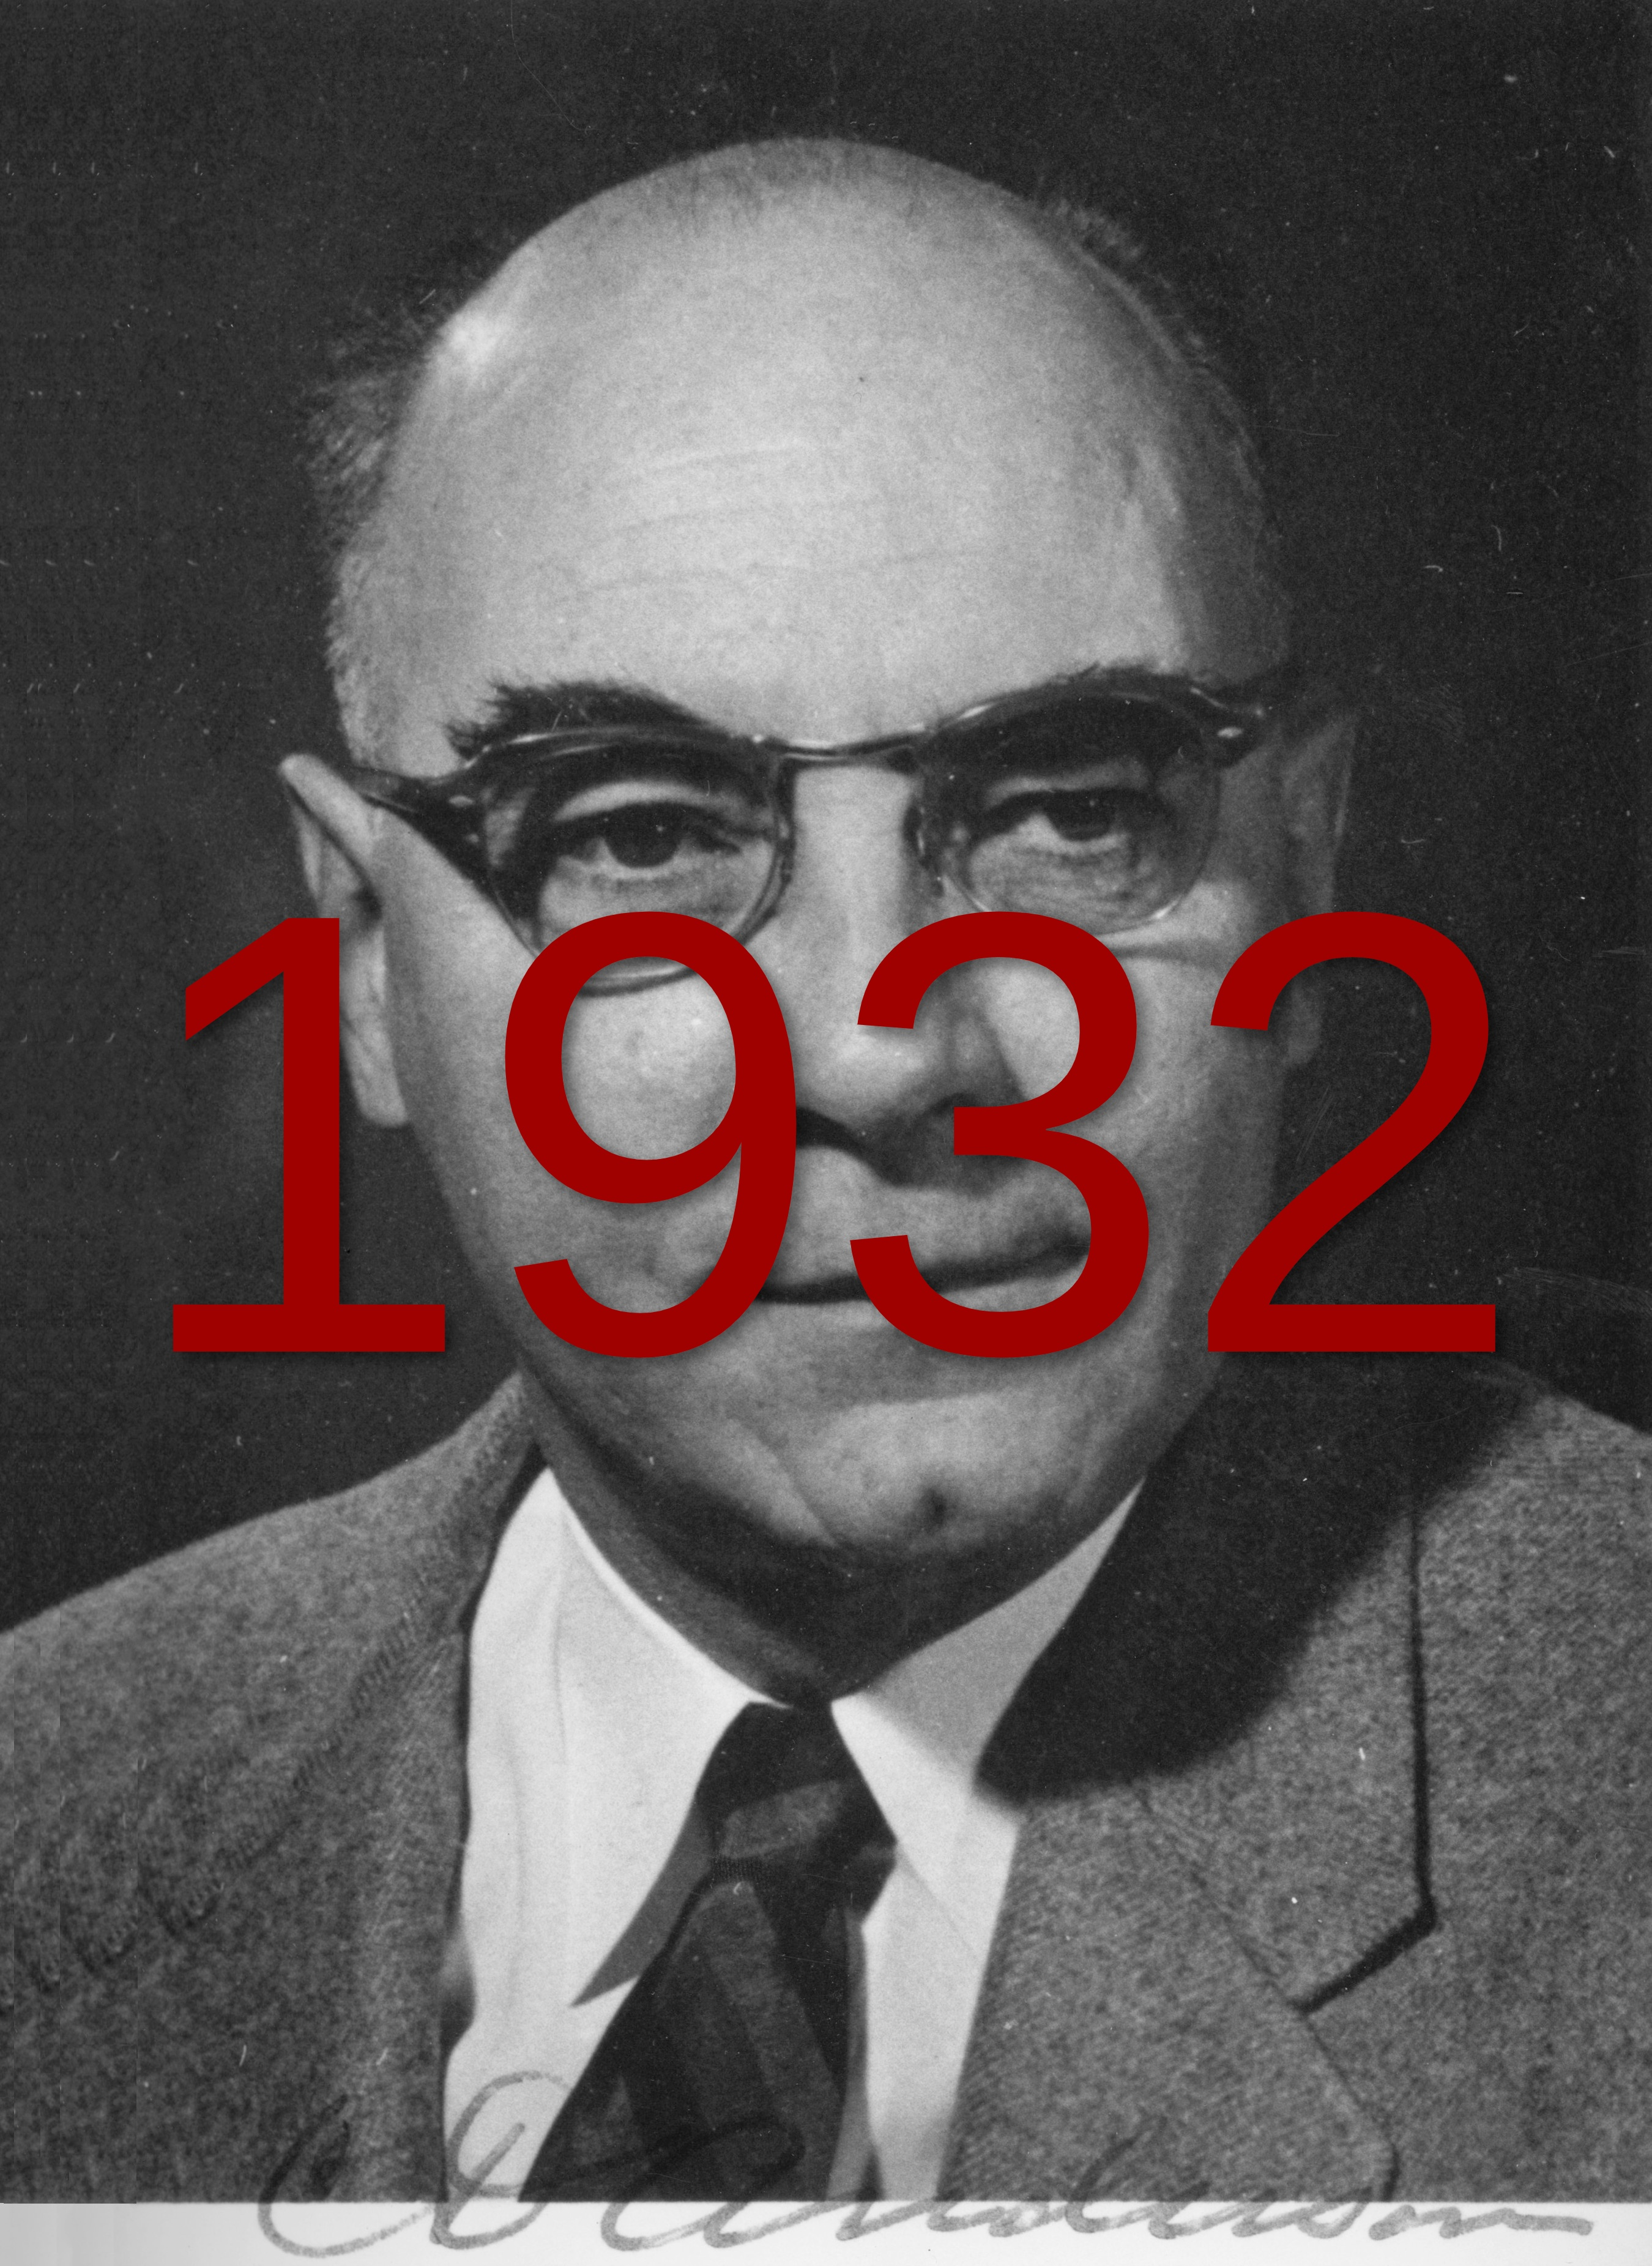
\includegraphics[width=0.4\textwidth]{../imgs/candersonp.jpg}
\label{fig:candersonpjpg}
  \end{figure}


\end{textblock*}

\begin{textblock*}{5cm}(3cm,0.2cm) % {block width} (coords)
\begin{figure}[H] 
  \centering
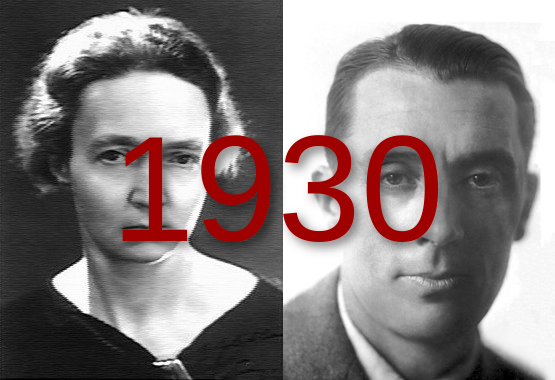
\includegraphics[width=0.8\textwidth]{../imgs/bcuriep.png}
\label{fig:bcurieppng}
  \end{figure}


\end{textblock*}

\begin{textblock*}{5cm}(6cm,0.2cm) % {block width} (coords)
\begin{figure}[H] 
  \centering
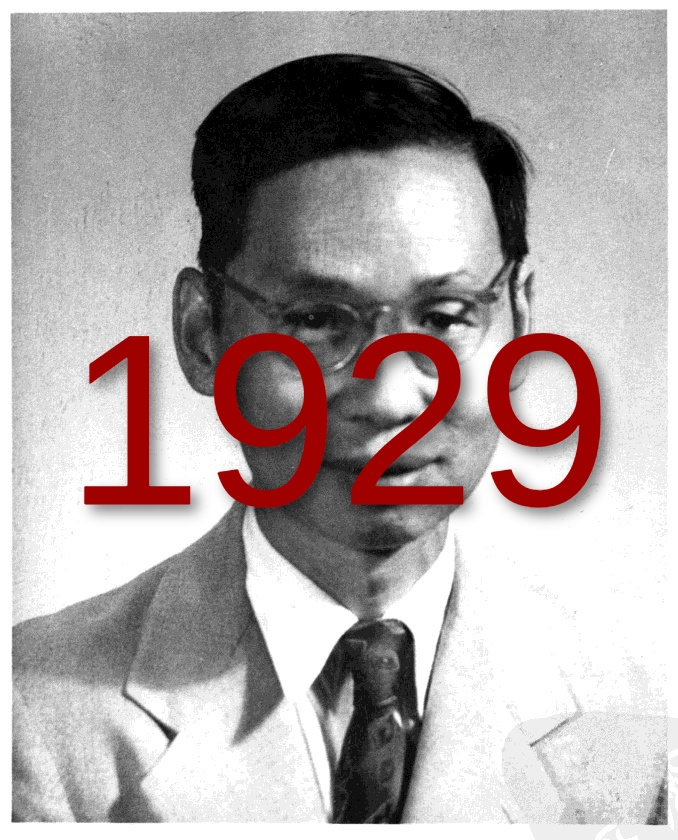
\includegraphics[width=0.4\textwidth]{../imgs/cchaop.jpg}
\label{fig:cchaopjpg}
  \end{figure}


\end{textblock*}

\begin{textblock*}{5cm}(8cm,0.2cm) % {block width} (coords)
\begin{figure}[H] 
  \centering
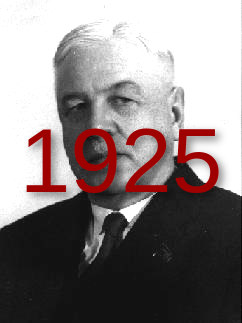
\includegraphics[width=0.4\textwidth]{../imgs/skobelp.png}
\label{fig:skobelppng}
  \end{figure}


\end{textblock*}







\vspace{3cm}
\begin{itemize}

    \item Detection of Antimatter

    \item Not extremely hard to detect, but deserved Nobel Prize

    \item Today:

\begin{itemize}

    \item fundamental building block of physics

    \item required to understand advanced chemistry/biology

    \item medical uses


\end{itemize}
    \item Also Today: Anomalies are sorely needed in Physics


\end{itemize}
\end{frame}




\begin{frame}[label=]
\frametitle{}
Instead of ~1000 Events/day$\Rightarrow$1 Petabyte/day

\begin{figure}[H] 
  \centering
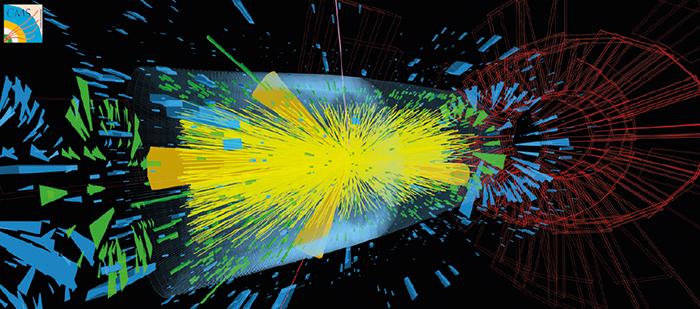
\includegraphics[width=1.0\textwidth]{../imgs/lhc_event2.jpg}
\label{fig:lhc_event2jpg}
  \end{figure}


$\Rightarrow$require computers
\end{frame}




\newpage
\section{Jet Anomaly}\label{sec:Jet Anomaly}
%{{{for_Jet Anomaly}}}

%new physics at the lhc
%introduce toptagging on this slide
\begin{frame}[label=Top Tagging]
\frametitle{Top Tagging}
\begin{columns}[c] % align columns
\begin{column}{0.48\textwidth}%.48
\begin{itemize}

    \item Looking at LHC jets (particle showers)

    \item Millions of jets, maybe some of them weird in some way

    \item But at most a few and in some unknown way

    \item So use ML to filter them out

    \item Usually tested by trying to find top jets in a qcd background


\end{itemize}
\end{column}%
\hfill%
\begin{column}{0.48\textwidth}%.48
\begin{figure}[H]
\begin{center}$
\begin{array}{c}
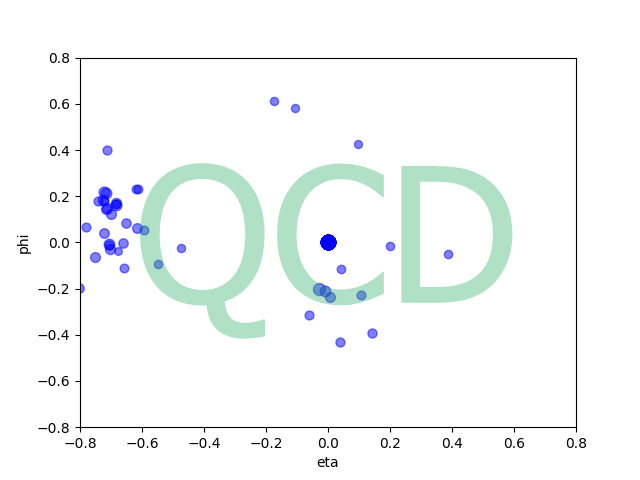
\includegraphics[width=0.8\textwidth]{../imgs/xoneqcd.png} \\
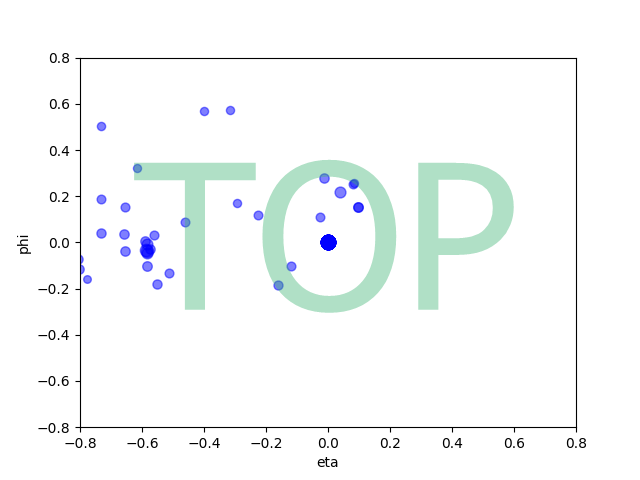
\includegraphics[width=0.8\textwidth]{../imgs/xonetop.png}
\end{array}$
\end{center}
\label{fig:xoneqcdpng}
\end{figure}

\end{column}%
\hfill%
\end{columns}

\end{frame}



%from file ../oan/presentation//data/02idea
\newpage
\section{Graph Autoencoder}\label{sec:Graph Autoencoder}
%{{{for_Graph Autoencoder}}}

\begin{frame}[label=]
\frametitle{}
\begin{columns}[c] % align columns
\begin{column}{0.48\textwidth}%.48
\begin{itemize}

    \item \href{https://arxiv.org/abs/1902.08570}{
ParticleNet
}

\begin{itemize}

    \item supervised

    \item Graph Neuronal Networks


\end{itemize}
    \item \href{https://arxiv.org/abs/1808.08979}{
Qcd Or What?
}

\begin{itemize}

    \item unsupervised

    \item Convolutional Networks


\end{itemize}

\end{itemize}
\end{column}%
\hfill%
\begin{column}{0.48\textwidth}%.48
\begin{itemize}

    \item Combine ideas from both

    \item Into a Graph Autoencoder


\end{itemize}
\end{column}%
\hfill%
\end{columns}

\end{frame}





%from file ../oan/presentation//data/03gae
\newpage
\section{Graph Autoencoder}\label{sec:Graph Autoencoder}
%{{{for_Graph Autoencoder}}}

\begin{frame}[label=]
\frametitle{}
\begin{columns}[c] % align columns
\begin{column}{0.48\textwidth}%.48
\begin{figure}[H] 
  \centering
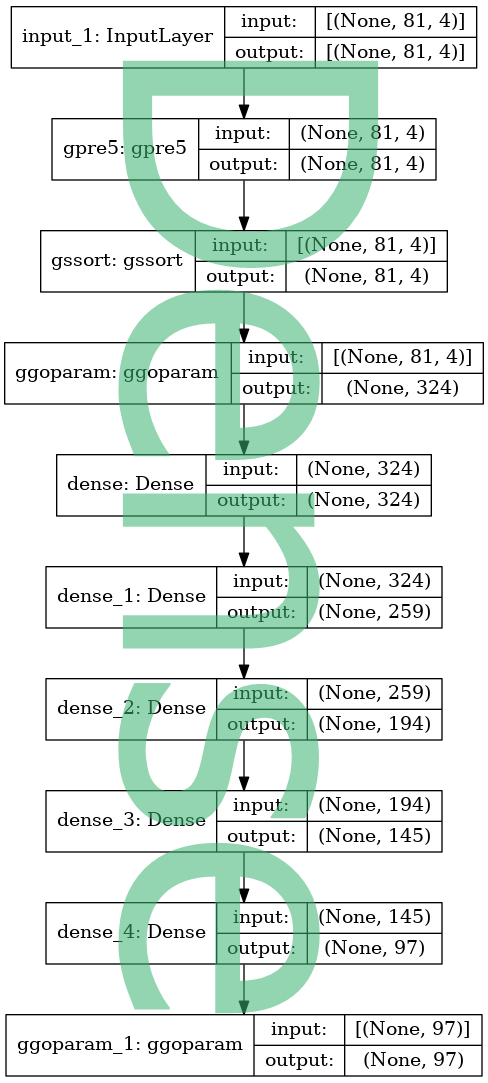
\includegraphics[height=0.9\textheight]{../imgs/xdenseencode.png}
\label{fig:xdenseencodepng}
  \end{figure}


\end{column}%
\hfill%
\begin{column}{0.48\textwidth}%.48
\begin{figure}[H] 
  \centering
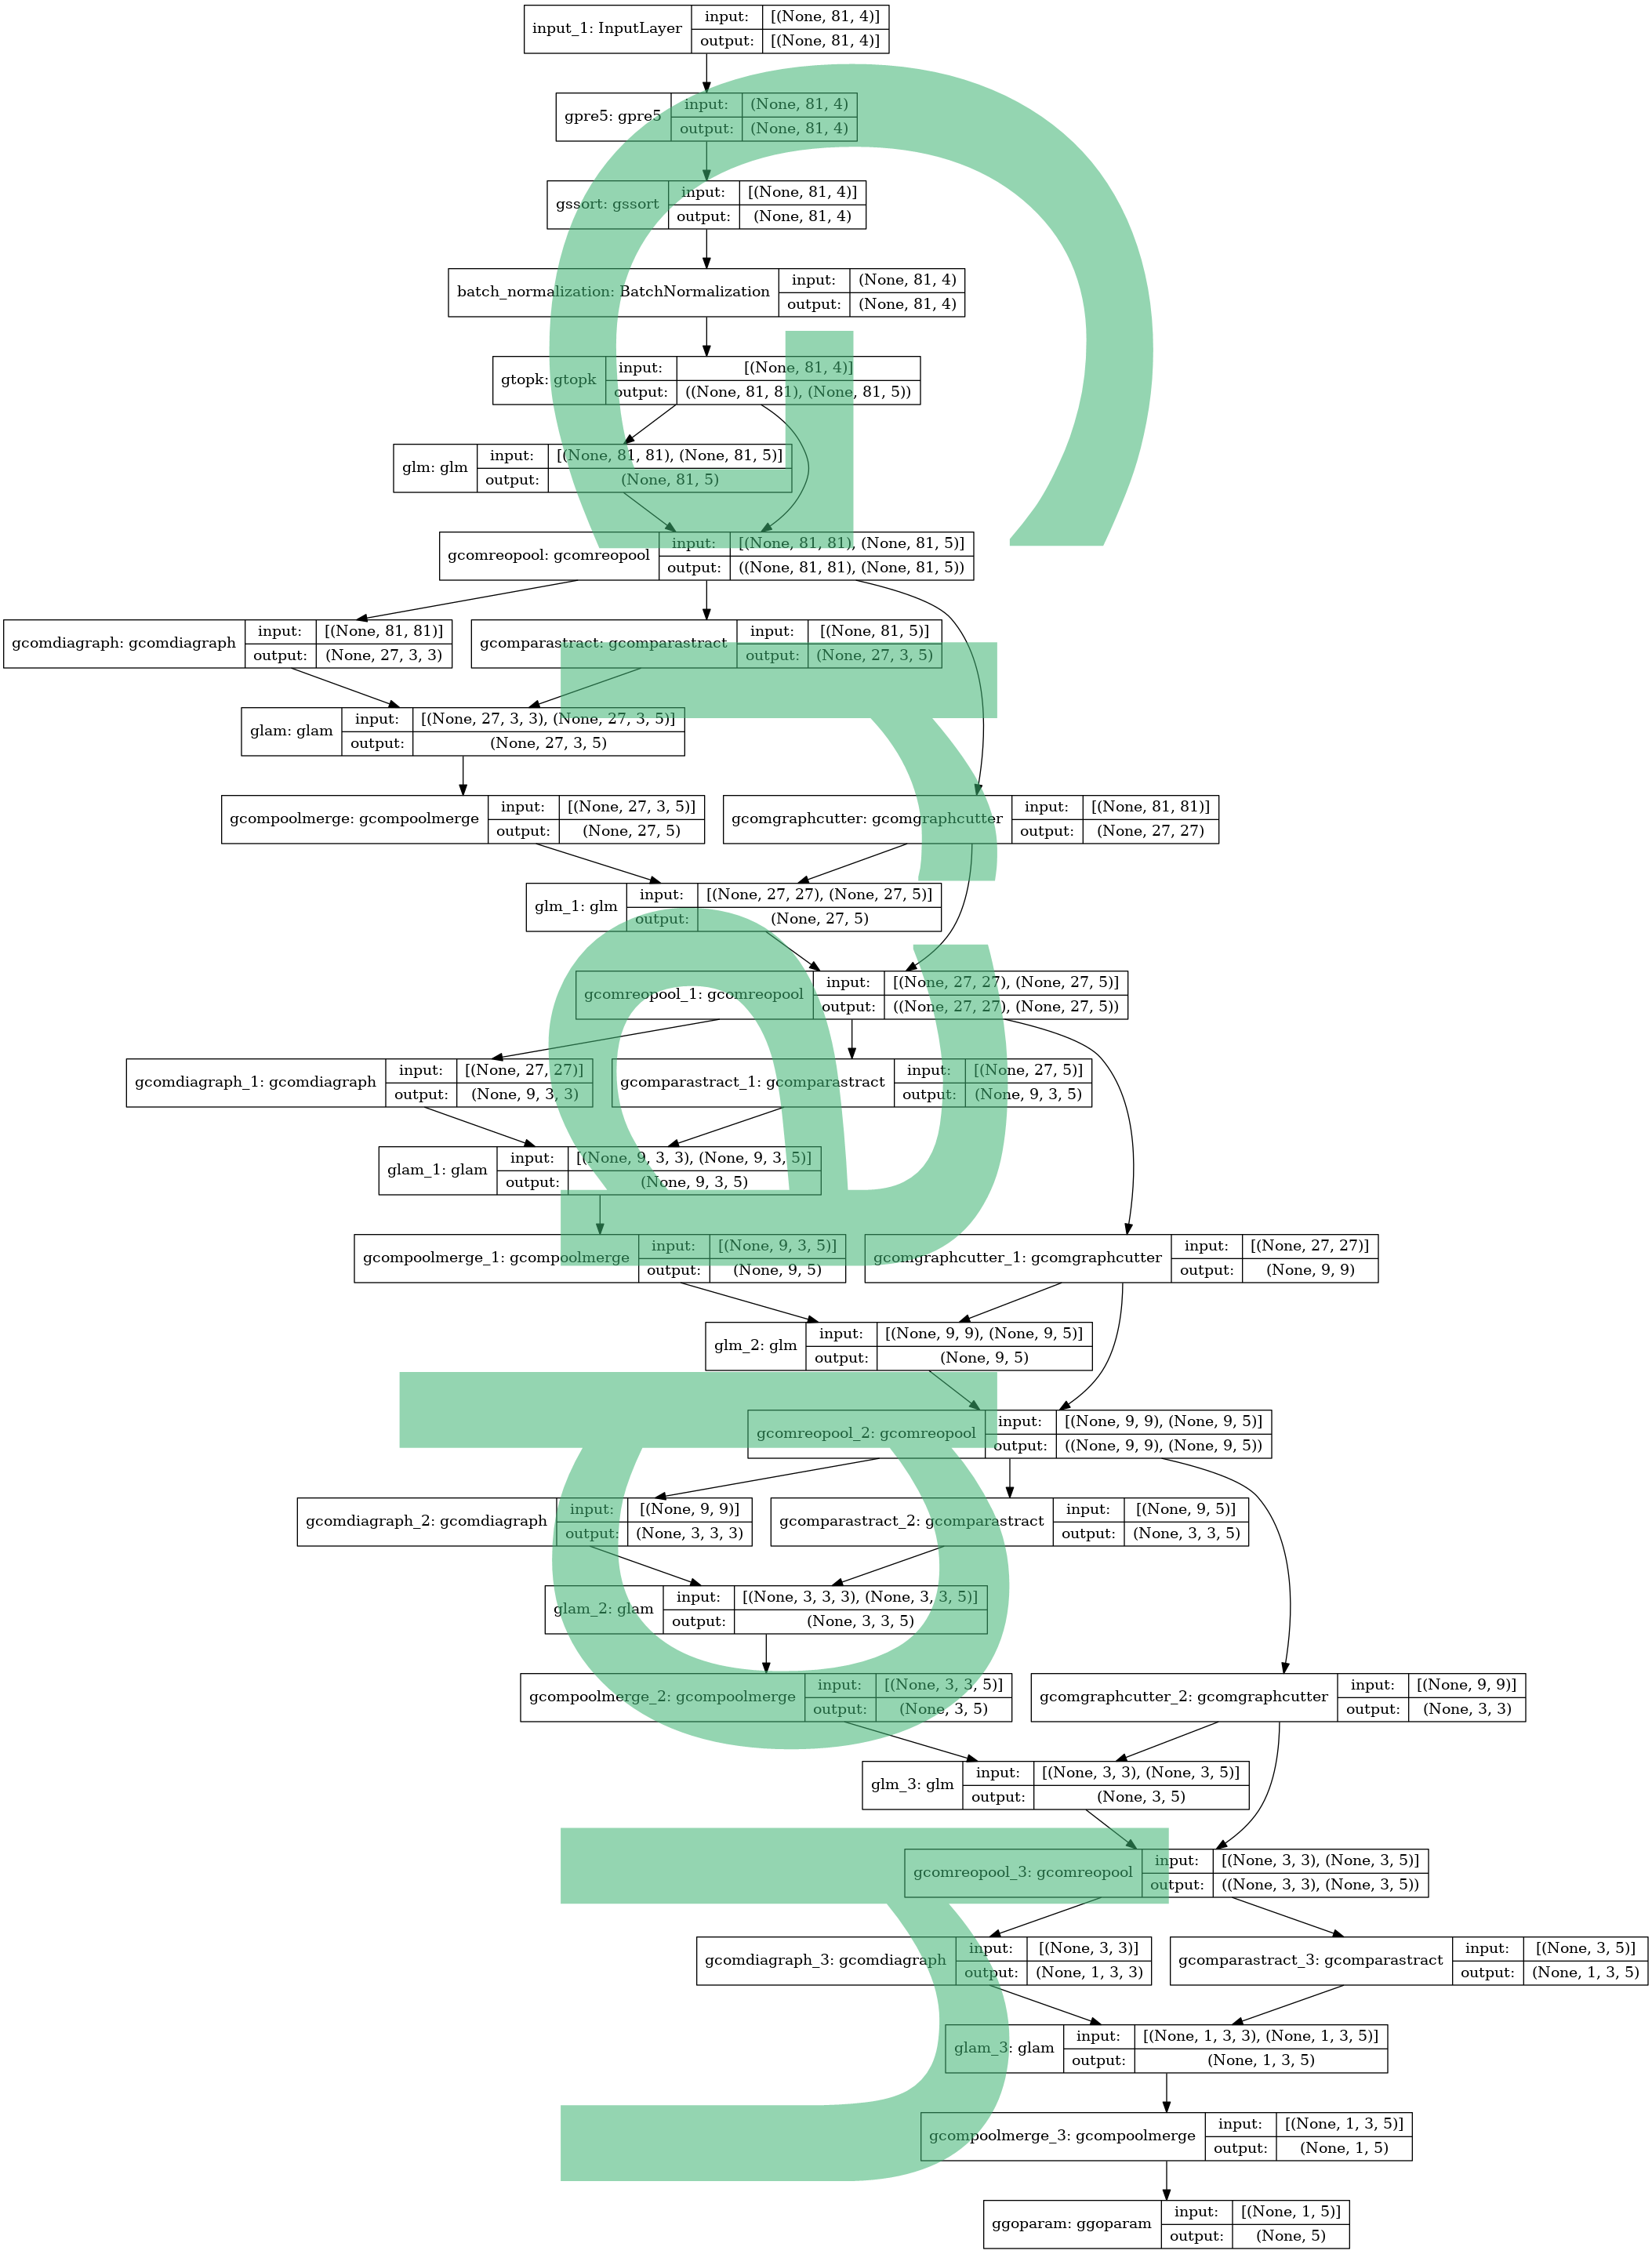
\includegraphics[height=0.9\textheight]{../imgs/xgraphencode.png}
\label{fig:xgraphencodepng}
  \end{figure}


\end{column}%
\hfill%
\end{columns}

\begin{textblock*}{5cm}(8.7cm,0.2cm) % {block width} (coords)
\begin{figure}[H] 
  \centering
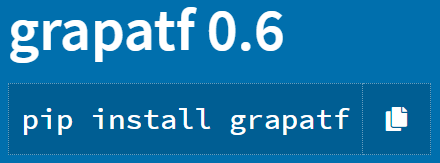
\includegraphics[width=0.6\textwidth]{../imgs/grapa.png}
\label{fig:grapapng}
  \end{figure}


\end{textblock*}

\end{frame}





%from file ../oan/presentation//data/04a
\newpage
\section{Graph Autoencoder}\label{sec:Graph Autoencoder}
%{{{for_Graph Autoencoder}}}

\begin{frame}[label=]
\frametitle{}
\begin{figure}[H] 
  \centering
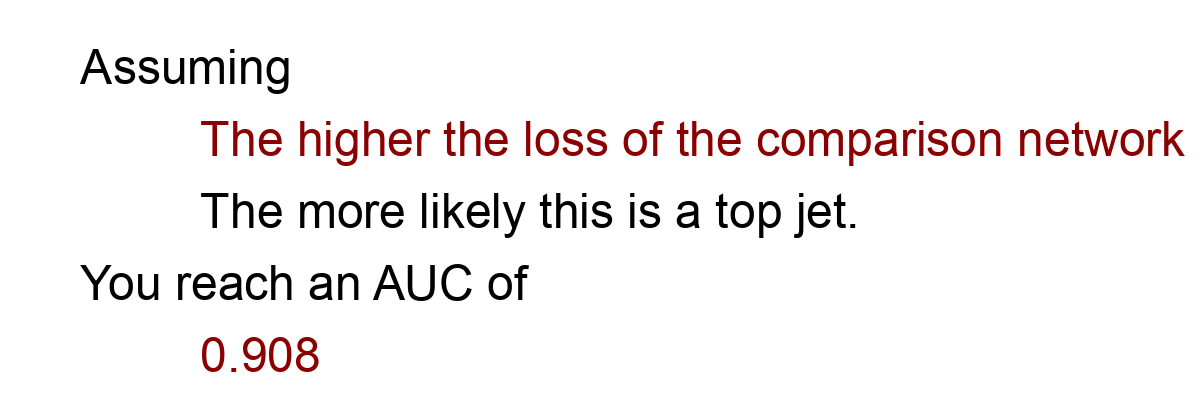
\includegraphics[width=0.9\textwidth]{../imgs/netresa}
\label{fig:netresa}
  \end{figure}


\begin{columns}[c] % align columns
\begin{column}{0.48\textwidth}%.48
\begin{itemize}

    \item Already fairly satisfied

    \item If I beat this, my graph networks work


\end{itemize}
\end{column}%
\hfill%
\begin{column}{0.48\textwidth}%.48
\begin{itemize}

    \item AUC score

    \item between 0 and 1, higher=better

    \item 1:perfect,0.5:random


\end{itemize}
\end{column}%
\hfill%
\end{columns}

\end{frame}





%from file ../oan/presentation//data/04b
\newpage
\section{Graph Autoencoder}\label{sec:Graph Autoencoder}
%{{{for_Graph Autoencoder}}}

\begin{frame}[label=]
\frametitle{}
\begin{figure}[H] 
  \centering
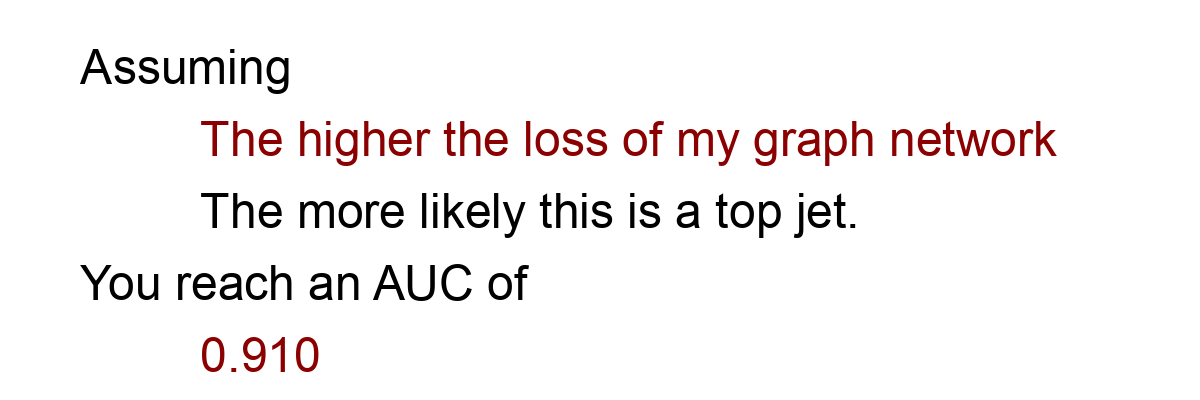
\includegraphics[width=0.9\textwidth]{../imgs/netresb}
\label{fig:netresb}
  \end{figure}


\begin{columns}[c] % align columns
\begin{column}{0.48\textwidth}%.48
\begin{itemize}

    \item So my network works

    \item But...


\end{itemize}
\end{column}%
\hfill%
\begin{column}{0.48\textwidth}%.48
\begin{itemize}

    \item AUC score

    \item between 0 and 1, higher=better

    \item 1:perfect,0.5:random


\end{itemize}
\end{column}%
\hfill%
\end{columns}

\end{frame}





%from file ../oan/presentation//data/04c
\newpage
\section{Graph Autoencoder}\label{sec:Graph Autoencoder}
%{{{for_Graph Autoencoder}}}

\begin{frame}[label=]
\frametitle{}
\begin{figure}[H] 
  \centering
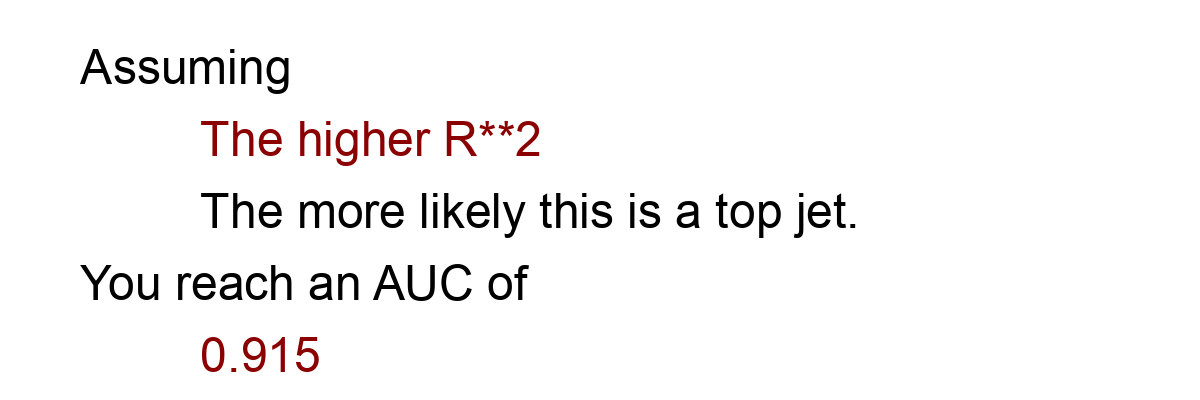
\includegraphics[width=0.9\textwidth]{../imgs/netresc}
\label{fig:netresc}
  \end{figure}


\begin{columns}[c] % align columns
\begin{column}{0.48\textwidth}%.48
\begin{itemize}

    \item trivial network

    \item best score yet


\end{itemize}
\end{column}%
\hfill%
\begin{column}{0.48\textwidth}%.48
\begin{itemize}

    \item AUC score

    \item between 0 and 1, higher=better

    \item 1:perfect,0.5:random


\end{itemize}
\end{column}%
\hfill%
\end{columns}

\end{frame}





%from file ../oan/presentation//data/05results
\newpage
\section{Results}\label{sec:Results}
%{{{for_Results}}}


\begin{frame}[label=Results]
\frametitle{Results}
\begin{columns}[c] % align columns
\begin{column}{0.48\textwidth}%.48
\begin{itemize}

    \item Why? Trivial difference between the jets we look at

    \item Width is measured by bad autoencoders

    \item Ae does the same as the radius but worse


\end{itemize}
\end{column}%
\hfill%
\begin{column}{0.48\textwidth}%.48
\begin{figure}[H] 
  \centering
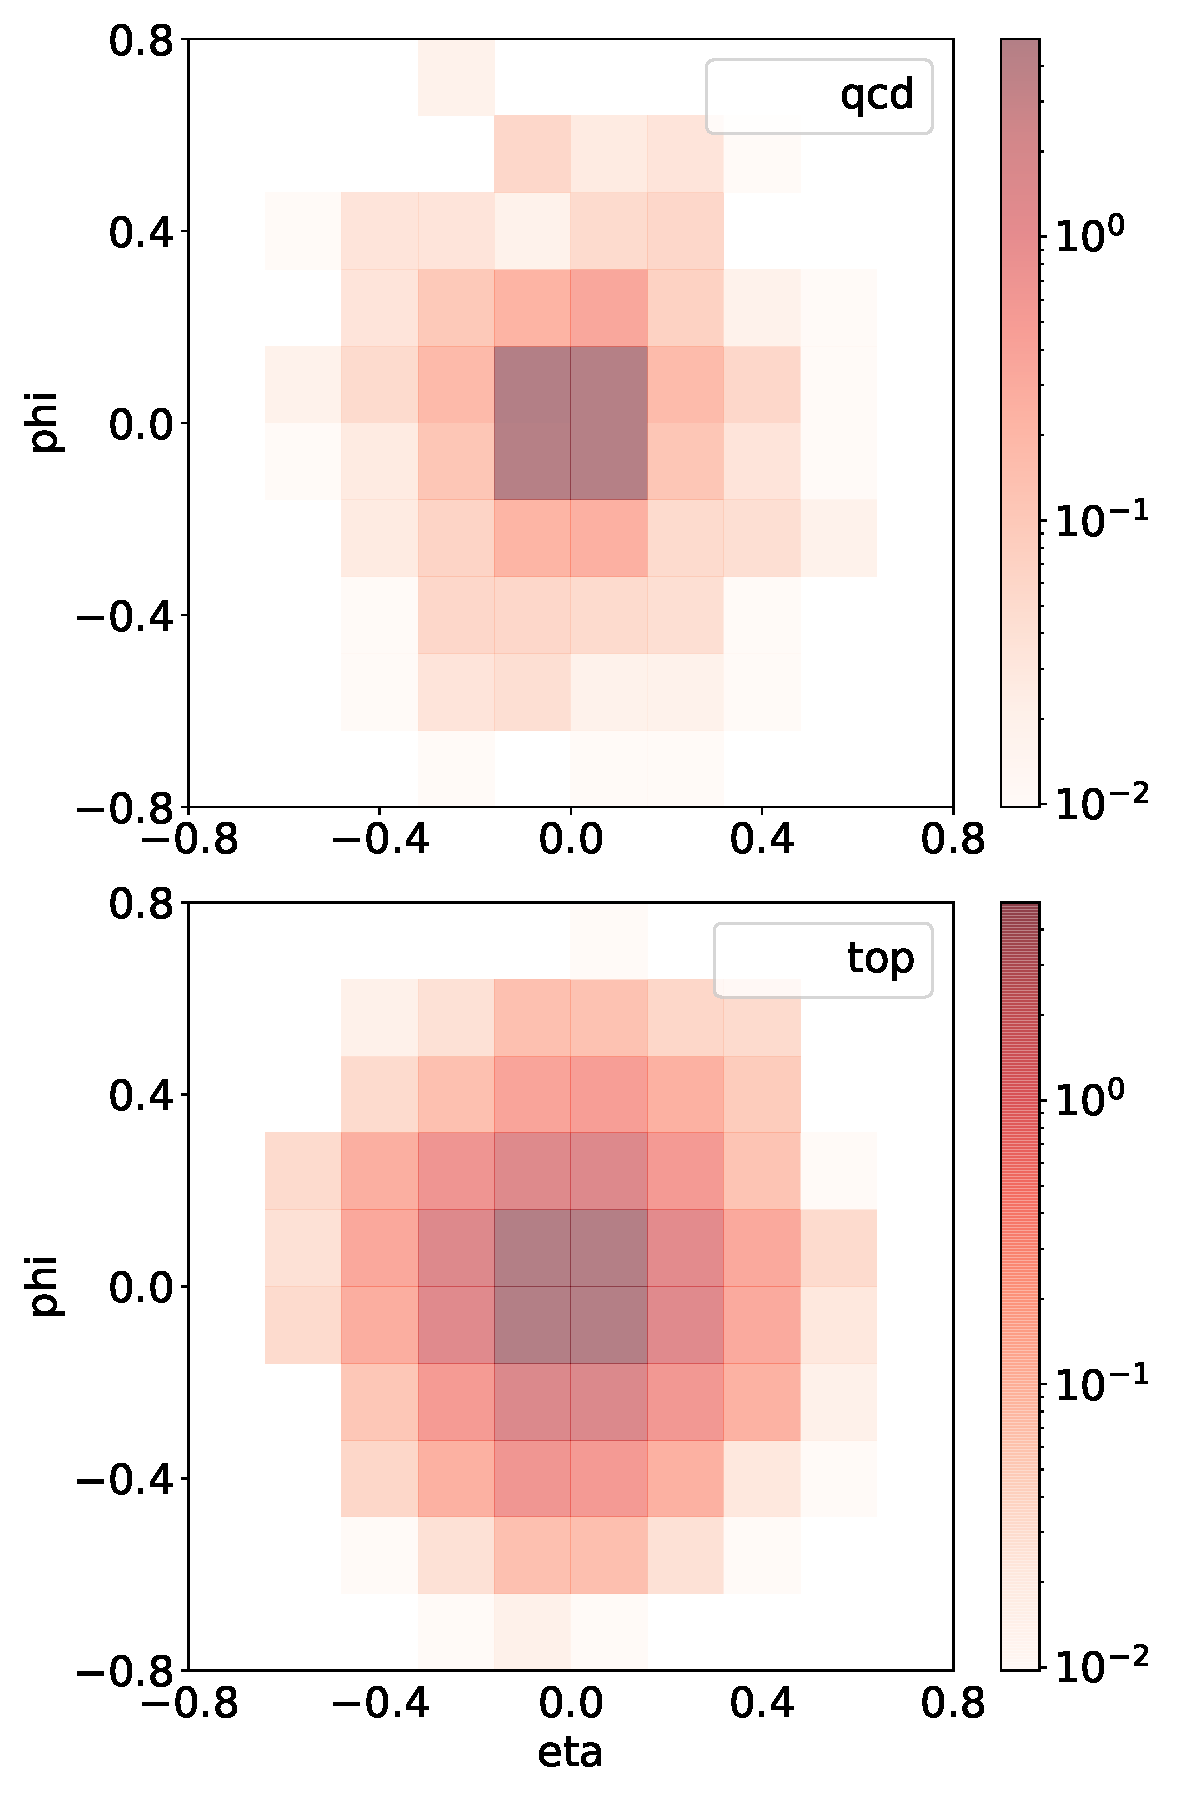
\includegraphics[width=0.90\textwidth]{../imgs/meanangle3}
\label{fig:meanangle3}
  \end{figure}


\end{column}%
\hfill%
\end{columns}

\end{frame}


\begin{frame}[label=data_0]
\frametitle{Results}
\begin{columns}[c] % align columns
\begin{column}{0.3\textwidth}%.48
\begin{itemize}

    \item The more blue the better, and if a pixel is red (dot) it is not detectable

    \item For the comparison work only 10(32)/56 are detectable

    \item useless, except for qcd vs top


\end{itemize}
\end{column}%
\hfill%
\begin{column}{0.68\textwidth}%.48
\begin{figure}[H] 
  \centering
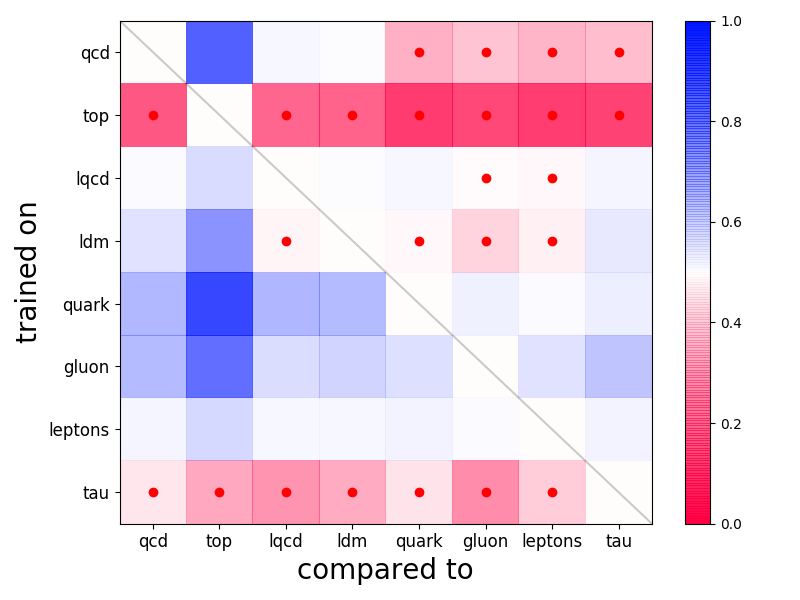
\includegraphics[width=0.95\textwidth]{../imgs/crossroc}
\label{fig:crossroc}
  \end{figure}


\end{column}%
\hfill%
\end{columns}

\end{frame}





%from file ../oan/presentation//data/06oo
\subsection{OneOff networks }\label{sec:OneOff networks}
%{{{for_OneOff networks}}}

\begin{frame}[label=oo_0]
\frametitle{OneOff Networks}
\begin{columns}[c] % align columns
\begin{column}{0.3\textwidth}%.48
\begin{itemize}

    \item So improve it using my own algorithm:

    \item Train a network to output a constant

    \item $loss = \left(f{\left(x \right)} - 1\right)^{2}$

    \item Anomalous data usually does not reproduce the same constant


\end{itemize}
\end{column}%
\hfill%
\begin{column}{0.68\textwidth}%.48
\begin{figure}[H] 
  \centering
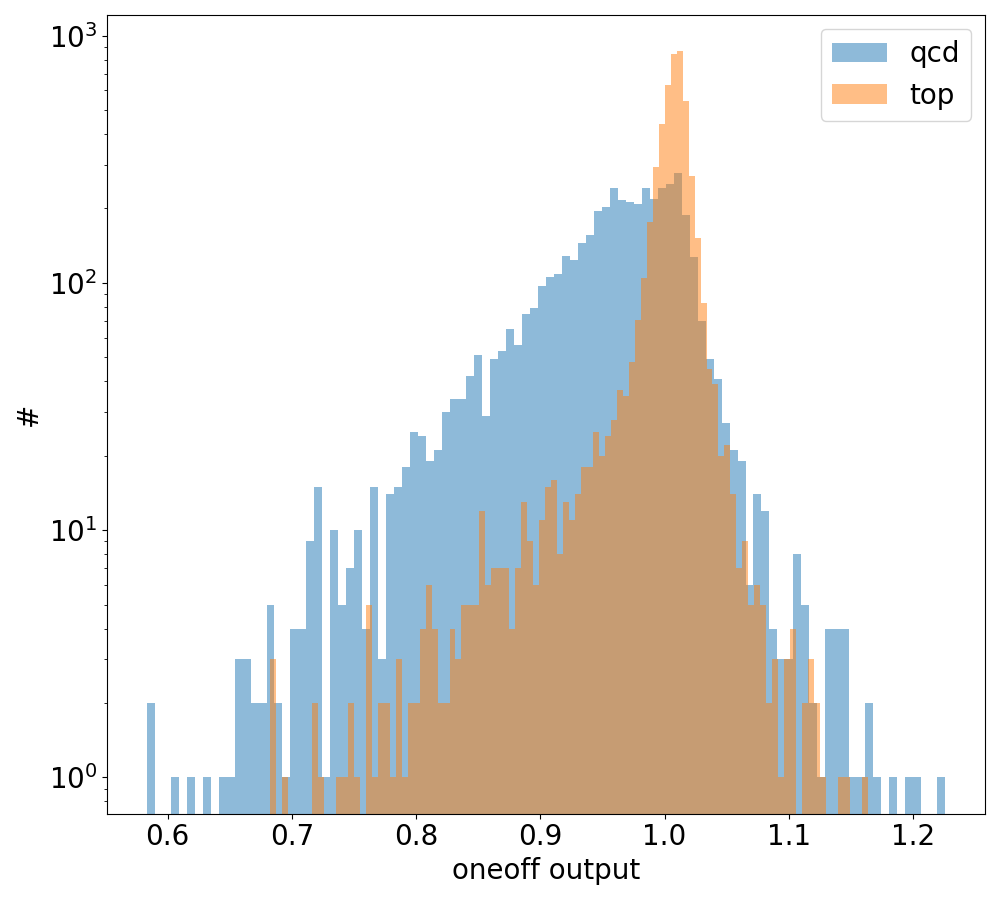
\includegraphics[width=0.85\textwidth]{../imgs/toosephist}
\label{fig:toosephist}
  \end{figure}


\end{column}%
\hfill%
\end{columns}

\end{frame}



%from file ../oan/presentation//data/07results
\newpage
\section{Results}\label{sec:Results}
%{{{for_Results}}}



\begin{frame}[label=data_0]
\frametitle{Results}
\begin{columns}[c] % align columns
\begin{column}{0.3\textwidth}%.48
\begin{itemize}

    \item The more blue the better, and if a pixel is red (dot) it is not detectable

    \item Quality is not final, but

    \item here do 48(52)/56 comparisons work


\end{itemize}
\end{column}%
\hfill%
\begin{column}{0.68\textwidth}%.48
\begin{figure}[H] 
  \centering
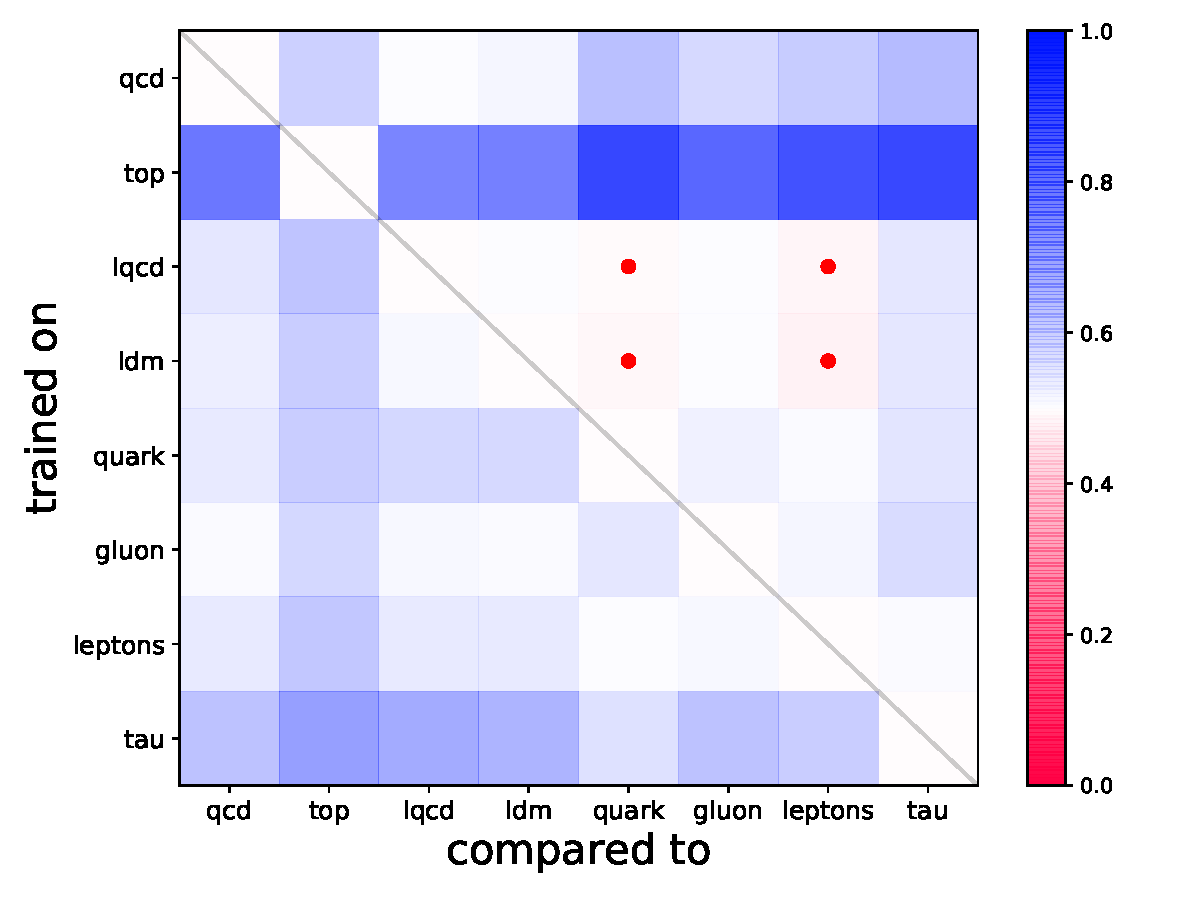
\includegraphics[width=0.95\textwidth]{../imgs/crosssep}
\label{fig:crosssep}
  \end{figure}


\end{column}%
\hfill%
\end{columns}

\end{frame}





%from file ../oan/presentation//data/08whyoo
\begin{frame}[label=]
\frametitle{}
\begin{columns}[c] % align columns
\begin{column}{0.48\textwidth}%.48
\begin{figure}[H] 
  \centering
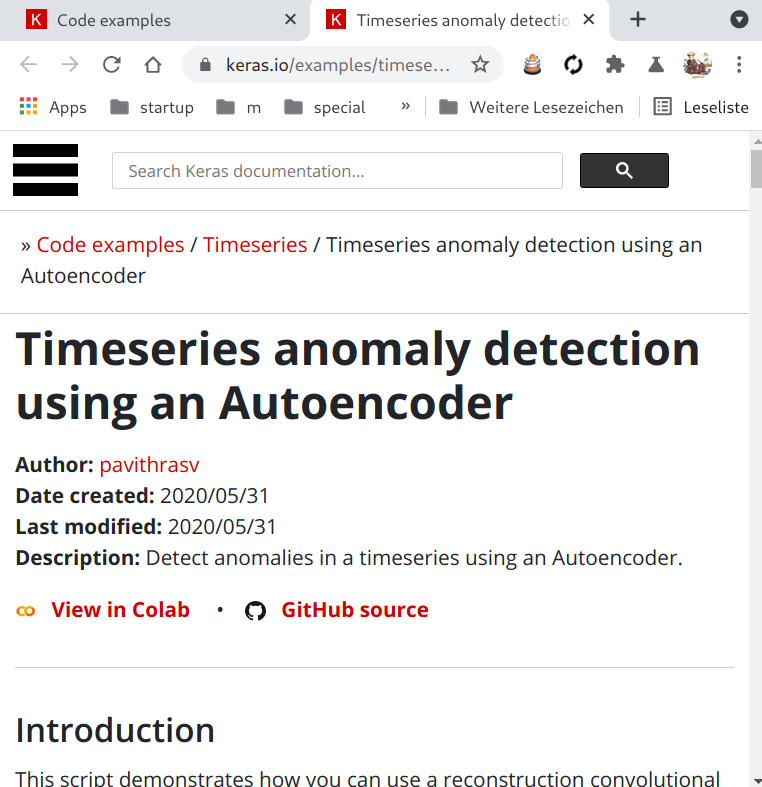
\includegraphics[width=1.0\textwidth]{../imgs/kanomal.png}
\label{fig:kanomalpng}
  \end{figure}


\end{column}%
\hfill%
\begin{column}{0.48\textwidth}%.48
\begin{table}[]
\begin{tabular}{lll}
          & Autoencoder & OneOff  \\
time      & 123s        & 22s      \\
AUC       & 99.6\%      & 99.92\% \\
$1 \cdot \frac{1}{1 - AUC}$ & 260         & 1290   
\end{tabular}
\end{table}


Will be used for the rest of this Presentation
\end{column}%
\hfill%
\end{columns}

\end{frame}



%from file ../oan/presentation//data/10newtitle
\newpage
\section{orthogonal anomaly detection}\label{sec:orthogonal anomaly detection}
%{{{for_orthogonal anomaly detection}}}



%from file ../oan/presentation//data/11what
\begin{frame}[label=Orthogonal Anomaly Detection]
\frametitle{Orthogonal Anomaly Detection}
\begin{columns}[c] % align columns
\begin{column}{0.48\textwidth}%.48
\begin{itemize}

    \item Usually nd input $\Rightarrow$ 1d anomaly score

    \item Why not nd input $\Rightarrow$ md anomaly score

    \item Retraining an anomaly detection algorithm provides about the same result

    \item Can you change this?

    \item And so create an multi-dimensional output anomaly detection algorithm

    \item $\Rightarrow$yes


\end{itemize}
\end{column}%
\hfill%
\begin{column}{0.48\textwidth}%.48
\begin{itemize}

    \item Create a general Framework for orthogonal anomaly detection

    \item Migth improve Generality, Interpretability and general Strength of anomaly detection


\end{itemize}
\end{column}%
\hfill%
\end{columns}

\end{frame}





%from file ../oan/presentation//data/12orthogonaloo
\begin{frame}[label=How]
\frametitle{How}
\begin{columns}[c] % align columns
\begin{column}{0.48\textwidth}%.48
\begin{itemize}

    \item Chance loss function

    \item From $loss = \left(f{\left(x \right)} - 1\right)^{2}$

    \item Too $\sum_{i<j} \lvert \left(\operatorname{f_{i}}{\left(x \right)} - 1\right) \cdot \left(\operatorname{f_{j}}{\left(x \right)} - 1\right) \rvert$


\end{itemize}
\end{column}%
\hfill%
\begin{column}{0.48\textwidth}%.48
$ \begin{bmatrix}
1 & 0.032 & -0.015 \\
0.032 & 1 & -0.14 \\
-0.015 & -0.14 & 1 
\end{bmatrix}  $
\end{column}%
\hfill%
\end{columns}

\end{frame}



%from file ../oan/presentation//data/13generality
\newpage
\section{Generality}\label{sec:Generality}
%{{{for_Generality}}}



\begin{frame}[label=Generality]
\frametitle{Generality}
\begin{itemize}

    \item Less important features can go hidden

    \item Also sometimes 2 errors can cancel each other out

    \item By having multiple outputs, you can reduce these effects

    \item Here I look at a different project, focussing on recurrent anomaly detection

    \item Same dataset as the keras example, but with another more complicated anomaly


\end{itemize}
\end{frame}



\begin{frame}[label=]
\frametitle{}
\begin{figure}[H] 
  \centering
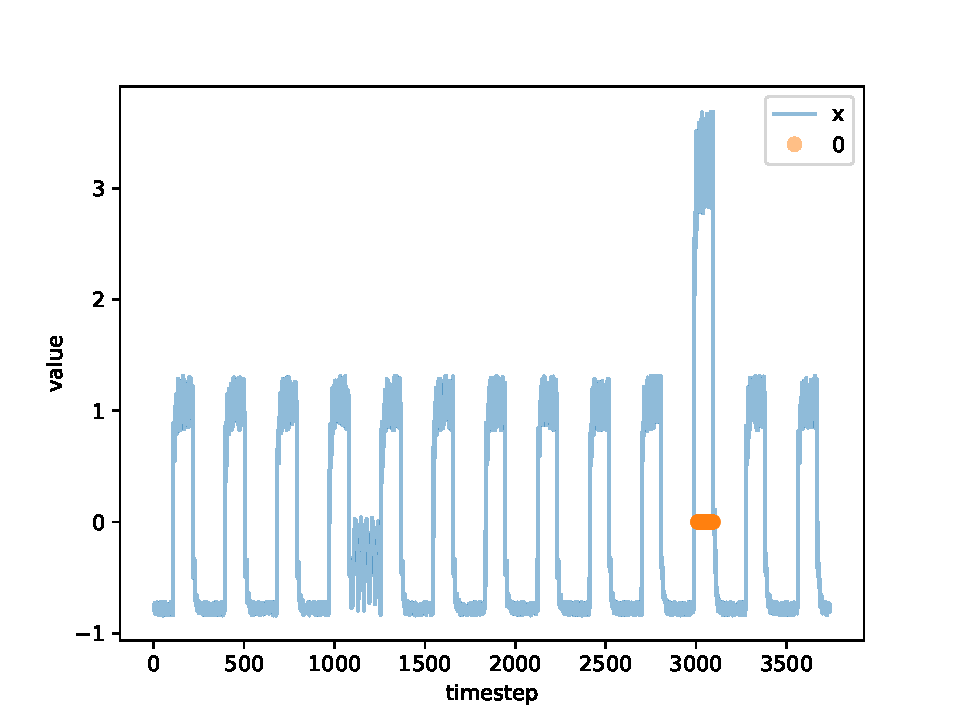
\includegraphics[width=0.9\textwidth]{../imgs/1d3}
\label{fig:1d3}
  \end{figure}


\end{frame}

\begin{frame}[label=]
\frametitle{}
\begin{figure}[H] 
  \centering
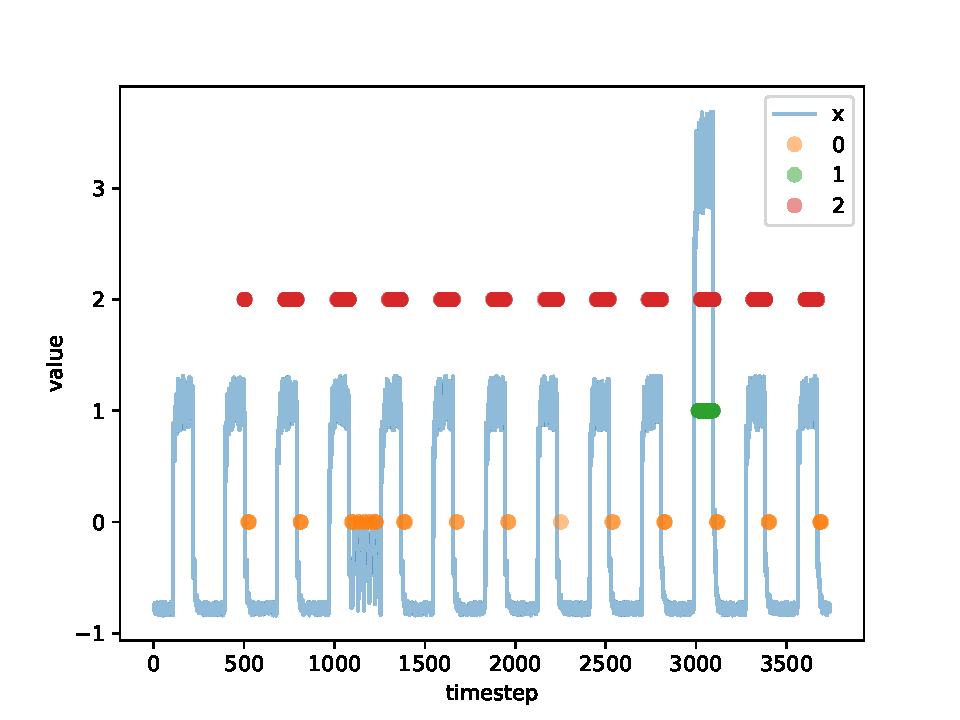
\includegraphics[width=0.9\textwidth]{../imgs/3d3}
\label{fig:3d3}
  \end{figure}


\end{frame}

\begin{frame}[label=]
\frametitle{}
\begin{figure}[H] 
  \centering
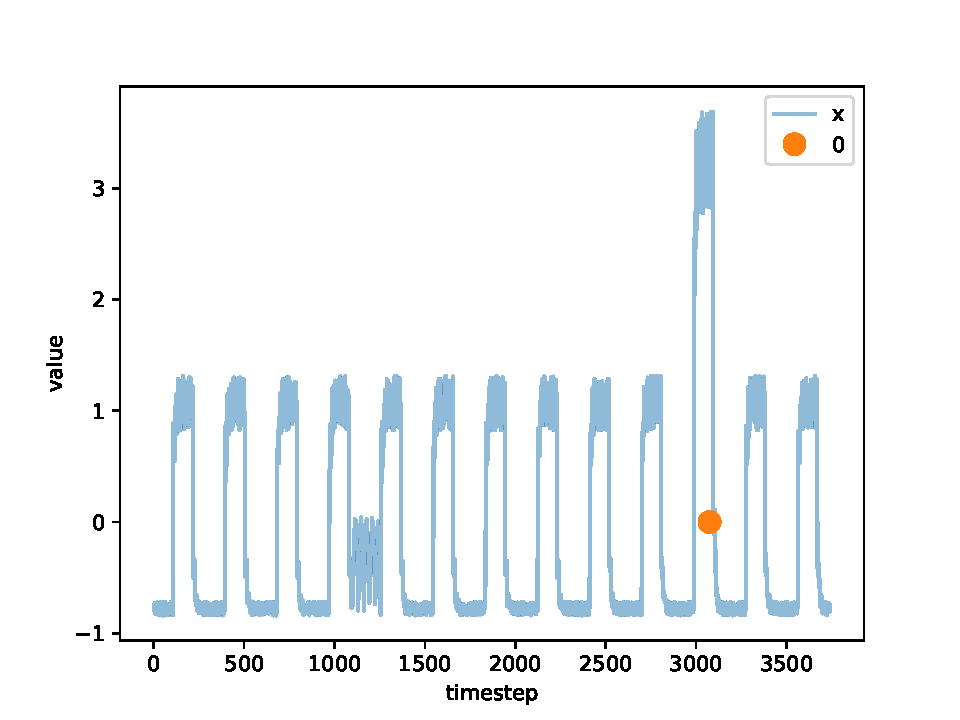
\includegraphics[width=0.9\textwidth]{../imgs/1d4}
\label{fig:1d4}
  \end{figure}


\end{frame}

\begin{frame}[label=]
\frametitle{}
\begin{figure}[H] 
  \centering
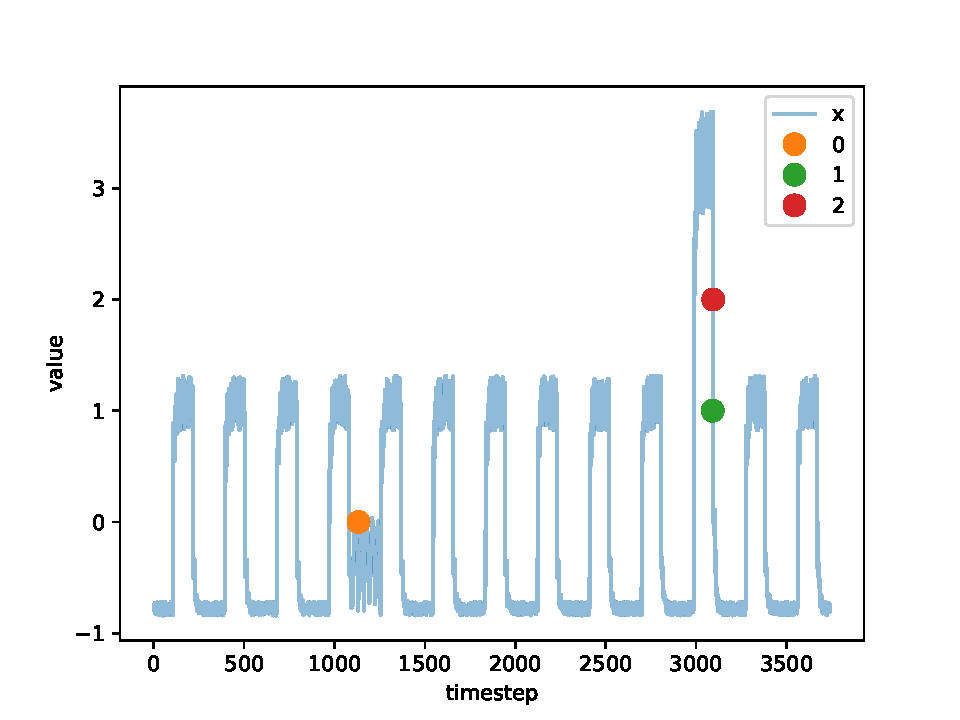
\includegraphics[width=0.9\textwidth]{../imgs/3d4}
\label{fig:3d4}
  \end{figure}


\end{frame}




%from file ../oan/presentation//data/14interpretability
\newpage
\section{Interpretability}\label{sec:Interpretability}
%{{{for_Interpretability}}}



\begin{frame}[label=Interpretability]
\frametitle{Interpretability}
\vspace{1cm}
\begin{itemize}

    \item By having an arbitrary number of output dimensions, you migth be able to find meaning in them

    \item Here looking at MNIST with 0 1 as normal case


\end{itemize}

\begin{figure}[H] 
  \centering
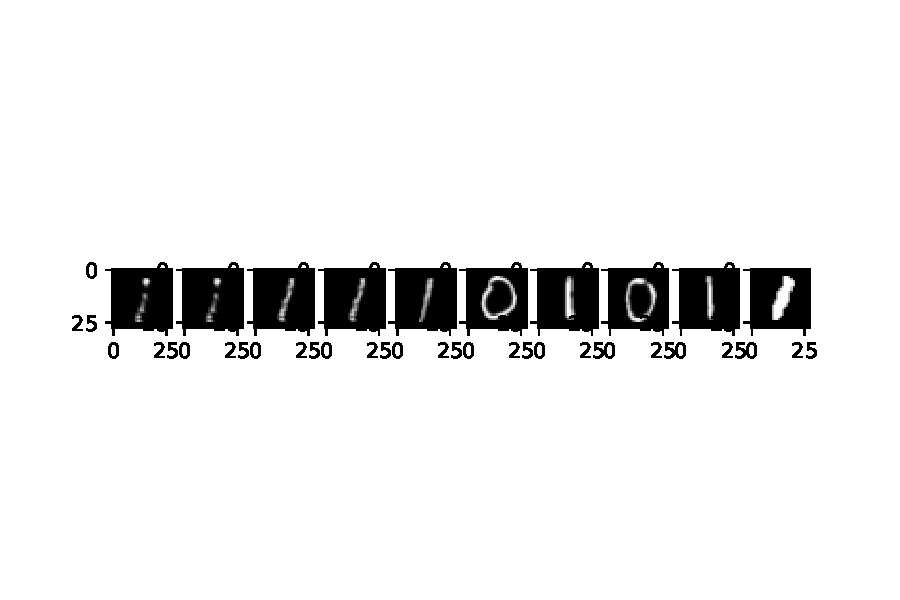
\includegraphics[width=0.8\textwidth]{../imgs/oneline}
\label{fig:oneline}
  \end{figure}


\end{frame}



\begin{frame}[label=]
\frametitle{}
\begin{figure}[H] 
  \centering
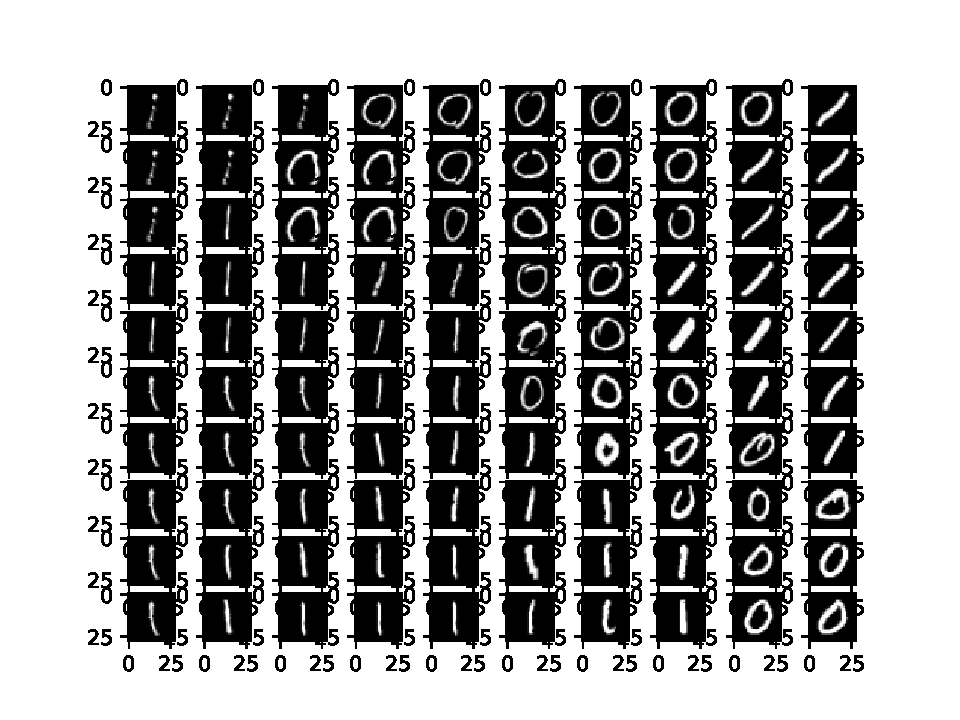
\includegraphics[width=0.9\textwidth]{../imgs/map}
\label{fig:map}
  \end{figure}


\end{frame}




%from file ../oan/presentation//data/15strength
\newpage
\section{Strength}\label{sec:Strength}
%{{{for_Strength}}}



\begin{frame}[label=Strength]
\frametitle{Strength}
\begin{itemize}

    \item Not ignoring (weak) features leads to better performance

    \item Also: this is able to combat the curse of dimensionality

    \item Here looking at one layer mnist anomaly detection (7 as normal class)

    \item generally really bad ($AUC = 0.65$)

    \item for comparison:2007.06963 reaches $0.982$


\end{itemize}
\end{frame}



\begin{frame}[label=]
\frametitle{}
\begin{figure}[H] 
  \centering
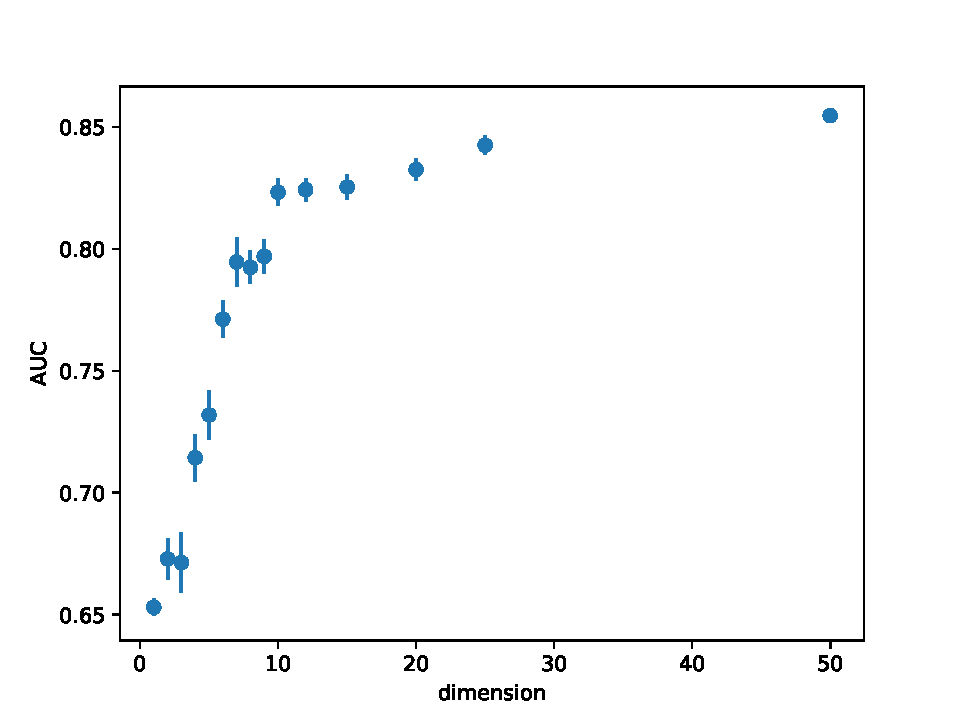
\includegraphics[width=0.9\textwidth]{../imgs/dimensional}
\label{fig:dimensional}
  \end{figure}


\end{frame}


\begin{frame}[label=]
\frametitle{}
\begin{figure}[H] 
  \centering
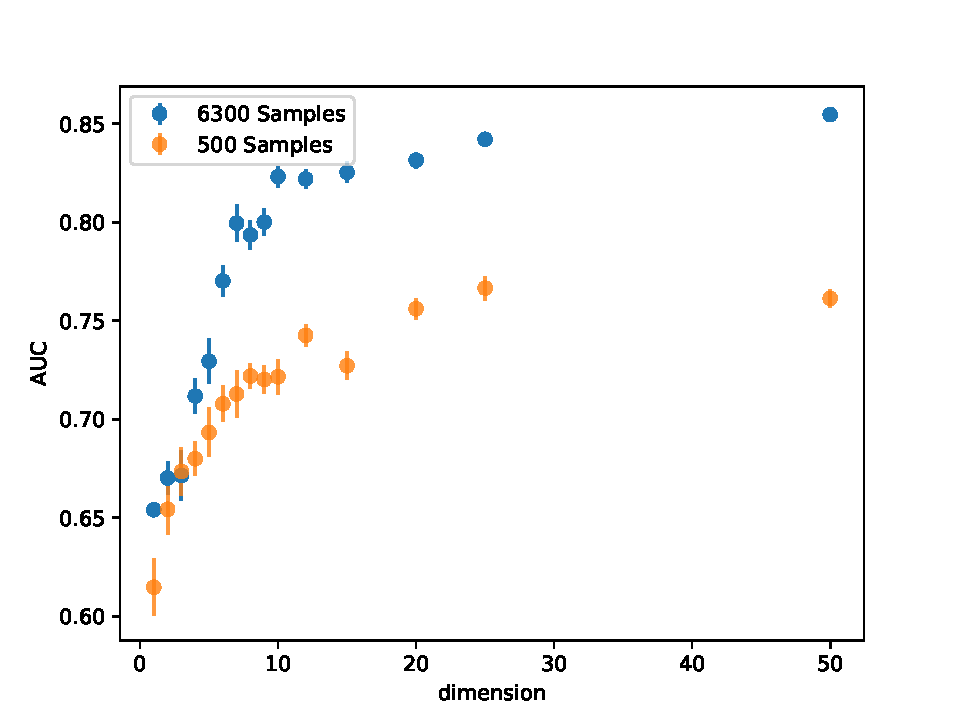
\includegraphics[width=0.9\textwidth]{../imgs/cdimensional}
\label{fig:cdimensional}
  \end{figure}


\end{frame}



%from file ../oan/presentation//data/16next
\newpage
\section{Whats next}\label{sec:Whats next}
%{{{for_Whats next}}}

\begin{frame}[label=Whats next]
\frametitle{Whats next}
\begin{columns}[c] % align columns
\begin{column}{0.48\textwidth}%.48
\begin{itemize}

    \item More efficient algorithm

    \item Try out other kinds of hard to find anomalies

    \item Better method of combining partial anomaly scores


\end{itemize}
\end{column}%
\hfill%
\begin{column}{0.48\textwidth}%.48
\begin{itemize}

    \item Other algorithms

\begin{itemize}

    \item Autoencoder, GAN based

    \item classical ones (knn, isolation forest, svm)


\end{itemize}
    \item Try to prevent Feature mixing for interpretability

    \item Ability to train supervised algorithms on unsupervised output


\end{itemize}
\end{column}%
\hfill%
\end{columns}

\end{frame}



%from file ../oan/presentation//data/17fin
\begin{frame}[noframenumbering]%%     1
\begin{center}
\Huge Thank You!
\end{center}
\end{frame}



%from folder ../oan/presentation//data/30backup


%from file ../oan/presentation//data/30backup/00section
\newpage
\appendix
%\addcontentsline{toc}{section}{Appendices}
%\section*{Appendices}

\newpage
\section{Backup}\label{sec:Backup}
%{{{for_Backup}}}



%from file ../oan/presentation//data/30backup/05gae
\subsection{Backup Graph Autoencoder }\label{sec:Backup Graph Autoencoder}
%{{{for_Backup Graph Autoencoder}}}

\begin{frame}[label=]
\frametitle{}
\begin{itemize}

    \item So here ParticleNet + QCDorWhat

    \item =Graph Autoencoder

    \item To do this, require:

\begin{itemize}

    \item An update step

\begin{itemize}

    \item already described


\end{itemize}

    \item something to reduce the number of nodes

    \item something to increase the number of nodes afterwards again


\end{itemize}

\end{itemize}
\end{frame}

\begin{frame}[label=Going from a big graph to a small graph]
\frametitle{Going from a big graph to a small graph}
\begin{itemize}

    \item similar to a Pooling operation for a convolutional network

    \item Seems simple enough but if you look at the literature

\begin{itemize}

    \item slow...and the benefits...are less clear (arXiv:1907.09000)

    \item advance...has lagged behind (arXiv:1907.00481)

    \item one cannot simply pool ... (arXiv:1806.08804)


\end{itemize}

\end{itemize}
\end{frame}

\begin{frame}[label=]
\frametitle{}
\begin{columns}[c] % align columns
\begin{column}{0.48\textwidth}%.48
\begin{figure}[H] 
  \centering
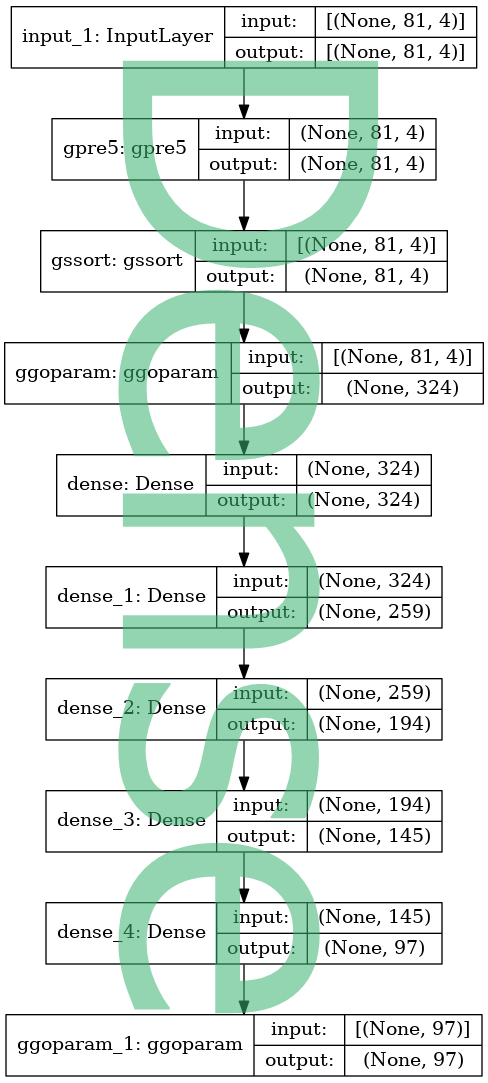
\includegraphics[height=0.9\textheight]{../imgs/xdenseencode.png}
\label{fig:xdenseencodepng}
  \end{figure}


\end{column}%
\hfill%
\begin{column}{0.48\textwidth}%.48
\begin{figure}[H] 
  \centering
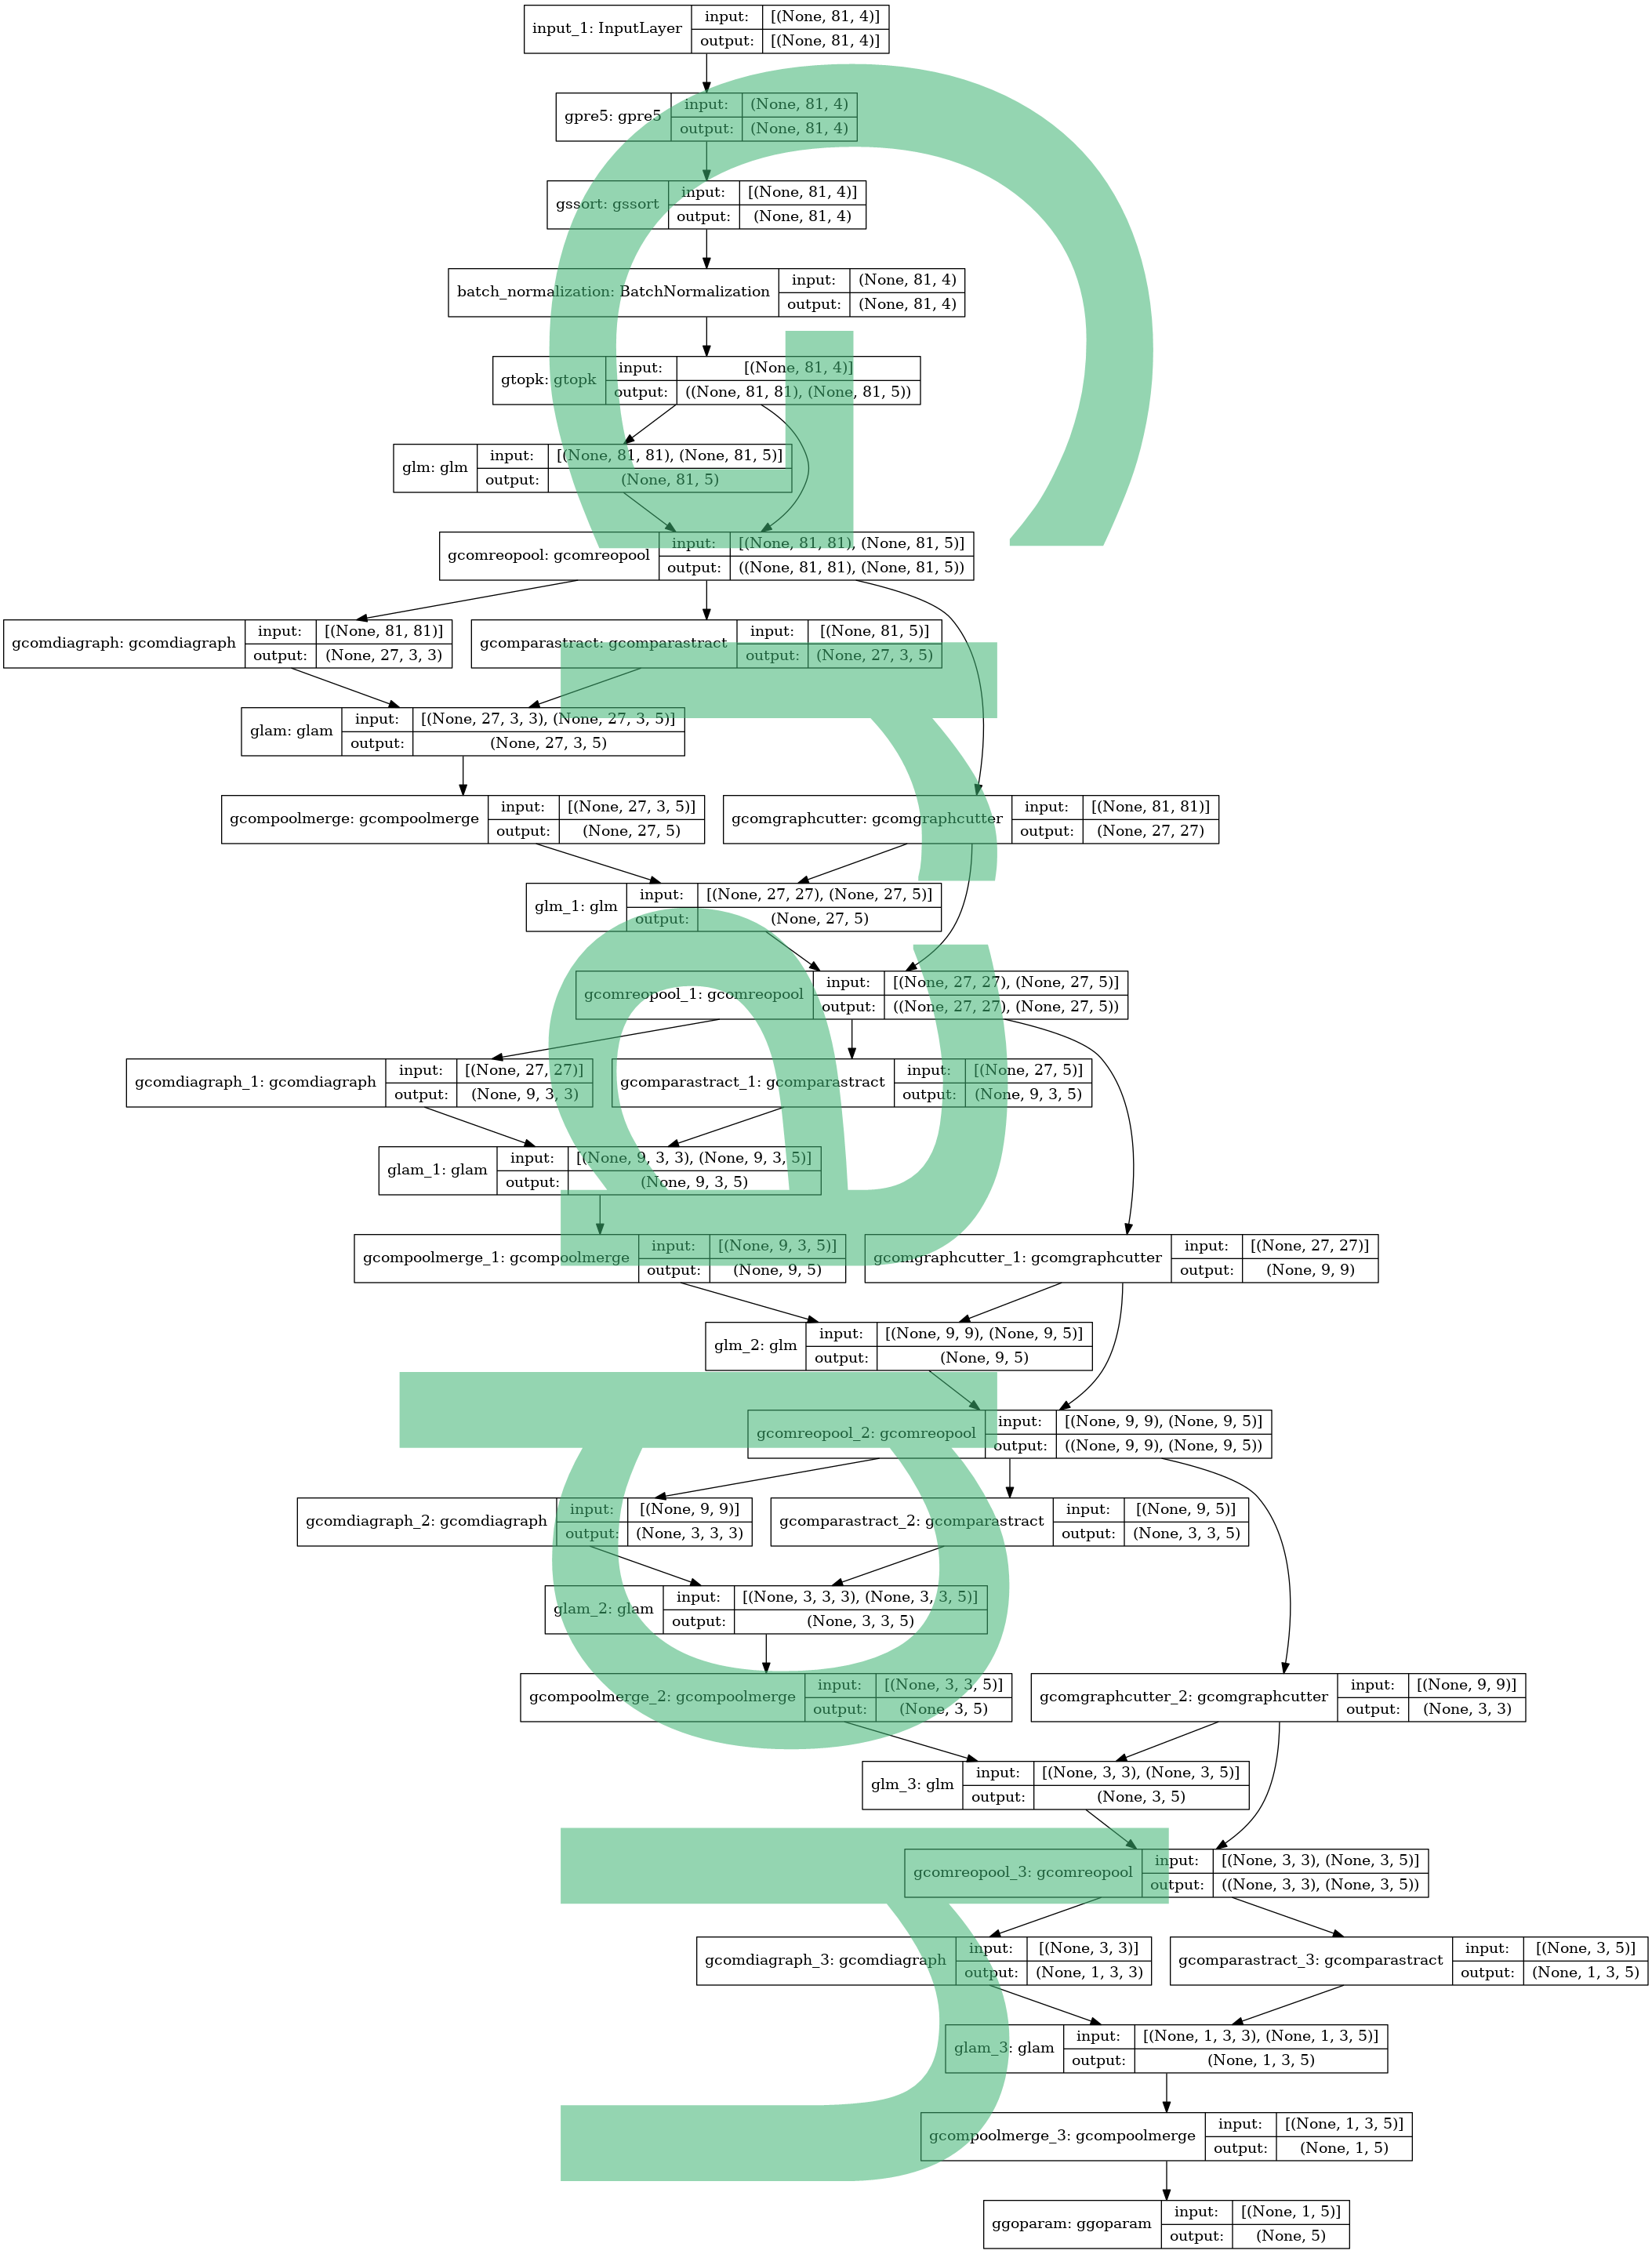
\includegraphics[height=0.9\textheight]{../imgs/xgraphencode.png}
\label{fig:xgraphencodepng}
  \end{figure}


\end{column}%
\hfill%
\end{columns}

\end{frame}

\begin{frame}[label=from a big graph to a small graph]
\frametitle{from a big graph to a small graph}
\begin{columns}[c] % align columns
\begin{column}{0.48\textwidth}%.48
\begin{itemize}

    \item project the graph on a learnable axis

    \item combine neigbour nodes on this axis

    \item relearn the graph or use a graph combination rule


\end{itemize}
\end{column}%
\hfill%
\begin{column}{0.48\textwidth}%.48
\begin{figure}[H] 
  \centering
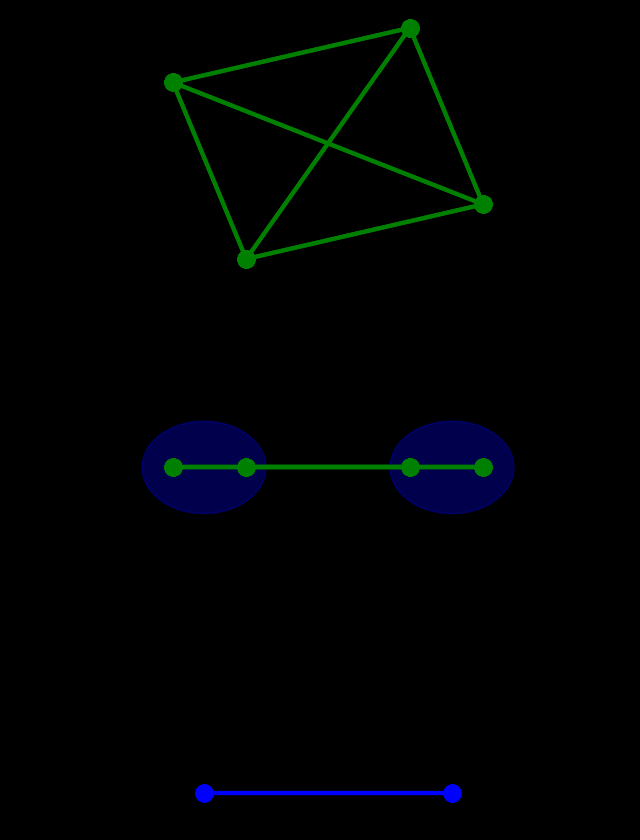
\includegraphics[width=0.9\textwidth]{../imgs/abiaa}
\label{fig:abiaa}
  \end{figure}


\end{column}%
\hfill%
\end{columns}

\end{frame}

\begin{frame}[label=from a small graph to a big graph]
\frametitle{from a small graph to a big graph}
\begin{columns}[c] % align columns
\begin{column}{0.48\textwidth}%.48
\begin{itemize}

    \item let each node grow into a learnable graph

    \item combine the new graphs with the existing one


\end{itemize}
\end{column}%
\hfill%
\begin{column}{0.48\textwidth}%.48
\begin{figure}[H] 
  \centering
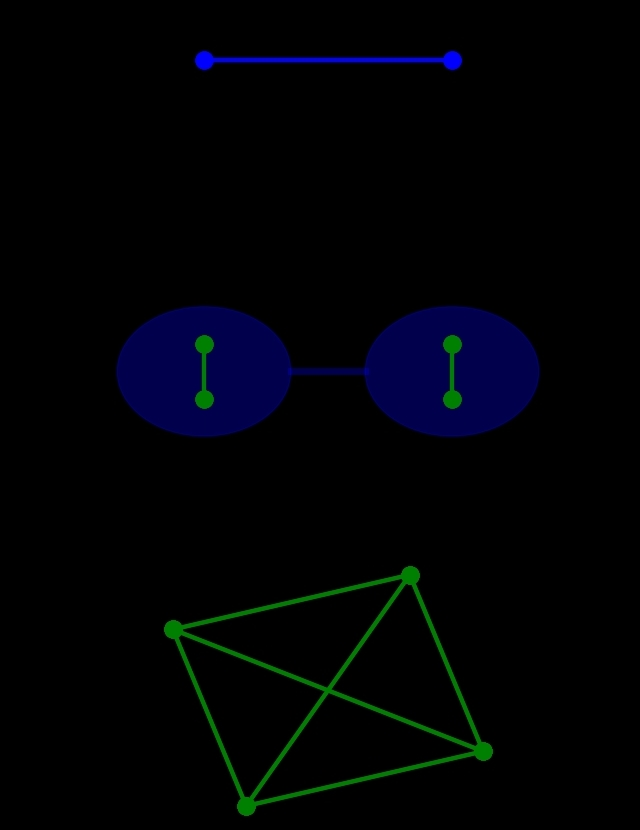
\includegraphics[width=0.9\textwidth]{../imgs/abibb}
\label{fig:abibb}
  \end{figure}


\end{column}%
\hfill%
\end{columns}

\end{frame}
















\end{document}
